\UseRawInputEncoding


%%%%%%%%%%%%%%%%%%%%%%%%%%%%%%%%%%%%%%%%%%%%%%%%%%%%%%%%%%%%%%%%%%%%%%%%%%%%%%%%
%% Settings
%%%%%%%%%%%%%%%%%%%%%%%%%%%%%%%%%%%%%%%%%%%%%%%%%%%%%%%%%%%%%%%%%%%%%%%%%%%%%%%%
%% Columns
\documentclass[final,3p,times,twocolumn]{elsarticle}
%% Use the options 1p,twocolumn; 3p; 3p,twocolumn; 5p; or 5p,twocolumn
%% for a journal layout:
%% \documentclass[final,1p,times]{elsarticle}
%% \documentclass[final,1p,times,twocolumn]{elsarticle}
%% \documentclass[final,3p,times]{elsarticle}
%% \documentclass[final,3p,times,twocolumn]{elsarticle}
%% \documentclass[final,5p,times]{elsarticle}
%% \documentclass[final,5p,times,twocolumn]{elsarticle}
%% \documentclass[preprint,review,12pt]{elsarticle}

%% Image width
\newlength{\imagewidth}
\newlength{\imagescale}
%% preamble
\usepackage[english]{babel}
\usepackage[table]{xcolor} % For coloring tables
\usepackage{booktabs} % For professional quality tables
\usepackage{colortbl} % For coloring cells in tables
\usepackage{amsmath, amssymb} % For mathematical symbols and environments
\usepackage{amsthm} % For theorem-like environments
\usepackage{lipsum} % just for sample text
\usepackage{natbib}
\usepackage{graphicx}
\usepackage{indentfirst}
\usepackage{bashful}
% for figures
\usepackage[margin=10pt,font=small,labelfont=bf,labelsep=endash]{caption}
\usepackage{graphicx}
\usepackage{calc}
% for tables
% \usepackage{xlsx2csv}
% \usepackage{csv2latex}
\usepackage[T1]{fontenc} % [REVISED]
\usepackage[utf8]{inputenc} % [REVISED]
\usepackage{hyperref}
\usepackage{accsupp}

%% Line numbers
\linespread{1.1}
% \linenumbers

% % Use accsupp package to make line numbers non-selectable/non-copyable in PDF
% \renewcommand\LineNumber{%
%   \BeginAccSupp{method=escape,ActualText={}}%
%   \thelinenumber\ %
%   \EndAccSupp{}%
% }

% % Ensure that listings package is loaded and configured if you want to include code listings
% \usepackage{listings}
% \lstset{
%   numbers=left,
%   numberstyle=\tiny,
%   stepnumber=1,
%   numbersep=5pt,
%   basicstyle=\ttfamily,
%   frame=tb,
%   framesep=5pt,
%   framexleftmargin=15pt,
%   backgroundcolor=\color{gray!10}
% }

% \makeatletter
% \def\lst@PlaceNumber{%
%   \llap{\normalfont
%     \pdfliteral direct{/Span<</ActualText()>>BDC}%
%     \lst@numberstyle{\thelstnumber}%
%     \pdfliteral direct{EMC}%
%     \kern\lst@numbersep%
%   }%
% }
% \makeatother
%%%%%%%%%%%%%%%%%%%%%%%%%%%%%%%%%%%%%%%%%%%%%%%%%%%%%%%%%%%%%%%%%%%%%%%%%%%%%%%%
%% Journal Name
%%%%%%%%%%%%%%%%%%%%%%%%%%%%%%%%%%%%%%%%%%%%%%%%%%%%%%%%%%%%%%%%%%%%%%%%%%%%%%%%
\journal{Heliyon}

%%%%%%%%%%%%%%%%%%%%%%%%%%%%%%%%%%%%%%%%%%%%%%%%%%%%%%%%%%%%%%%%%%%%%%%%%%%%%%%%
%% Document Starts
%%%%%%%%%%%%%%%%%%%%%%%%%%%%%%%%%%%%%%%%%%%%%%%%%%%%%%%%%%%%%%%%%%%%%%%%%%%%%%%%
\begin{document}


%%%%%%%%%%%%%%%%%%%%%%%%%%%%%%%%%%%%%%%%%%%%%%%%%%%%%%%%%%%%%%%%%%%%%%%%%%%%%%%%
%% frontmatter
%%%%%%%%%%%%%%%%%%%%%%%%%%%%%%%%%%%%%%%%%%%%%%%%%%%%%%%%%%%%%%%%%%%%%%%%%%%%%%%%
\begin{frontmatter}
\begin{highlights}
\pdfbookmark[1]{Highlights}{highlights}

\item Neural trajectories in the hippocampus exhibited greater variability during a working memory (WM) task compared to those in the entorhinal cortex and amygdala regions.

\item The distance of neural trajectories between encoding and retrieval states in the hippocampus was memory-load dependent during a WM task.


\item Hippocampal neural trajectories fluctuated between the encoding and retrieval states in a task-dependent manner during both baseline and sharp-wave ripple (SWR) periods.

\item Hippocampal neural trajectories shifted from encoding to retrieval states during SWR period.

\end{highlights}\title{
Hippocampal neural fluctuations between memory encoding and retrieval states during a working memory task in humans: Encoding-to-retrieval shift during sharp-wave ripples
}

\author[1]{Yusuke Watanabe\corref{cor1}}
\author[2,3,4]{Yuji Ikegaya}
\author[1,5]{Takufumi Yanagisawa}

\address[1]{Institute for Advanced Cocreation studies, Osaka University, 2-2 Yamadaoka, Suita, 565-0871, Osaka, Japan}
\address[2]{Graduate School of Pharmaceutical Sciences, The University of Tokyo, 7-3-1 Hongo, Tokyo, 113-0033, Japan}
\address[3]{Institute for AI and Beyond, The University of Tokyo, 7-3-1 Hongo, Tokyo, 113-0033, Japan}
\address[4]{Center for Information and Neural Networks, National Institute of Information and Communications Technology, 1-4 Yamadaoka, Suita City, 565-0871, Osaka, Japan}
\address[5]{Department of Neurosurgery, Osaka University Graduate School of Medicine, 2-2 Yamadaoka, Osaka, 565-0871, Japan}

\cortext[cor1]{Corresponding author. Tel: +81-6-6879-3652}
% \end{title*}%%Graphical abstract
%\pdfbookmark[1]{Graphical Abstract}{graphicalabstract}        
%\begin{graphicalabstract}
%\includegraphics{grabs}
%\end{graphicalabstract}
\begin{abstract}
\pdfbookmark[1]{Abstract}{abstract}

Working memory (WM) is indispensable for numerous cognitive functions, although the underlying neural mechanisms have not been fully elucidated. While the hippocampus and sharp-wave ripple complexes (SWRs) -- brief, synchronous neural events within the hippocampus -- are acknowledged for their importance in memory consolidation and retrieval, their association with WM tasks remains unclear. The present study posits that hippocampal multiunit activity patterns, in concert with SWRs, manifest distinct dynamics during WM tasks. We analyzed a dataset comprising intracranial electroencephalogram recordings from the medial temporal lobe (MTL) of nine epilepsy patients engaged in an eight-second Sternberg task. Gaussian-process factor analysis was utilized to extract low-dimensional neural representations, or 'trajectories', within MTL regions during the WM task. Our results reveal that the hippocampus demonstrates the most significant fluctuation in neural trajectory relative to the entorhinal cortex and amygdala. Furthermore, trajectories' dissimilarity measured between encoding and retrieval phases is dependent on memory load. Notably, hippocampal trajectories fluctuate during the retrieval phase and exhibit task-dependent shifts between encoding and retrieval states, both during baseline and SWR events. This fluctuation transitions from encoding to retrieval states in the presence of SWRs. These findings reinforce the pivotal role of the hippocampus in WM tasks and suggest a new hypothesis: the hippocampus alters its functional state from encoding to retrieval during SWRs.

\end{abstract}% \pdfbookmark[1]{Keywords}{keywords}                
\begin{keyword}
working memory \sep WM \sep memory load \sep hippocampus \sep sharp-wave ripples \sep SWR \sep humans
\end{keyword}
\end{frontmatter}

%%%%%%%%%%%%%%%%%%%%%%%%%%%%%%%%%%%%%%%%%%%%%%%%%%%%%%%%%%%%%%%%%%%%%%%%%%%%%%%%
%% main
%%%%%%%%%%%%%%%%%%%%%%%%%%%%%%%%%%%%%%%%%%%%%%%%%%%%%%%%%%%%%%%%%%%%%%%%%%%%%%%%
%%%%%%%%%%%%%%%%%%%%%%%%%%%%%%%%%%%%%%%%%%%%%%%%%%%%%%%%%%%%%%%%%%%%%%%%%%%%%%%% 
%% Introduction
%%%%%%%%%%%%%%%%%%%%%%%%%%%%%%%%%%%%%%%%%%%%%%%%%%%%%%%%%%%%%%%%%%%%%%%%%%%%%%%% 
\section{Introduction}
Working memory (WM) is crucial in everyday life; however, its neural mechanism has yet to be fully elucidated. Specifically, the role of the hippocampus, an essential brain region contributing to memory has been an ongoing topic \cite{scoville_loss_1957} \cite{squire_legacy_2009}  \cite{boran_persistent_2019} \cite{kaminski_persistently_2017} \cite{kornblith_persistent_2017} \cite{faraut_dataset_2018} \cite{borders_hippocampus_2022} \cite{li_functional_2023} \cite{dimakopoulos_information_2022}. Understanding the hippocampus' role in working memory is instrumental in deepening our knowledge of cognitive processes, ultimately aiding in developing cognitive training strategies and interventions.
\\
\indent
It is known that a transient and synchronous oscillation called sharp-wave ripple (SWR) \cite{buzsaki_hippocampal_2015} is associated with various cognitive functions, including memory replay \cite{wilson_reactivation_1994} \cite{nadasdy_replay_1999} \cite{lee_memory_2002} \cite{diba_forward_2007} \cite{davidson_hippocampal_2009}, memory consolidation \cite{girardeau_selective_2009} \cite{ego-stengel_disruption_2010} \cite{fernandez-ruiz_long-duration_2019} \cite{kim_corticalhippocampal_2022}, memory recall \cite{wu_hippocampal_2017} \cite{norman_hippocampal_2019} \cite{norman_hippocampal_2021}, and neural plasticity \cite{behrens_induction_2005} \cite{norimoto_hippocampal_2018}. Thus, SWR might be a fundamental representation of processing in the hippocampus and contribute to working memory performances. However, investigations into the effects of SWRs on working memory remain infrequent (\cite{jadhav_awake_2012} and limited to rodent models using navigation tasks, in which precise timings of memory acquisition and recall are not separated.
\\
\indent
Moreover, it is getting discovered that hippocampal neurons exhibit low-dimensional representations during WM tasks. For instance, the firing patterns of place cells \cite{okeefe_hippocampus_1971} \cite{okeefe_place_1976} \cite{ekstrom_cellular_2003} \cite{kjelstrup_finite_2008} \cite{harvey_intracellular_2009} in the hippocampus were embedded within a dynamic, nonlinear three-dimensional hyperbolic geometry in rodent \cite{zhang_hippocampal_2022}. Furthermore, grid cells in the entorhinal cortex (EC) --- the primary gateway to the hippocampus \cite{naber_reciprocal_2001} \cite{van_strien_anatomy_2009} \cite{strange_functional_2014} --- exhibited toroidal topology during exploration \cite{gardner_toroidal_2022}. However, again, these experiments are limited to spatial navigation tasks in rodents so that the temporal resolution of WM tasks is constrained. Moreover, whther these findings are generalized to humans and beyond navigation tasks, are not investigated yet.
\\
\indent
Given these backgrounds, in this study, we investigated the hypothesis that hippocampal neurons exhibit distinct representations in low-dimensional spaces as 'neural trajectory' during WM tasks, with a specific focus on SWR periods. To test this hypothesis, we utilized a dataset of patients performing an eight-second Sternberg task with high temporal resolution (1 s for fixation, 2 s for encoding, 3 s for maintenance, and 2 s for retrieval) while their intrachranial electroencephalography signals (iEEG) in the medial temporal lobe (MTL) were recorded \cite{boran_dataset_2020}. To explore low-dimensional neural trajectories, we employed Gaussian-process factor analysis (GPFA) based on multiunit activities, a proven tool for the analysis of neural population dynamics \cite{yu_gaussian-process_2009}.
\label{sec:introduction}

%%%%%%%%%%%%%%%%%%%%%%%%%%%%%%%%%%%%%%%%%%%%%%%%%%%%%%%%%%%%%%%%%%%%%%%%%%%%%%%%
%% Methods
%%%%%%%%%%%%%%%%%%%%%%%%%%%%%%%%%%%%%%%%%%%%%%%%%%%%%%%%%%%%%%%%%%%%%%%%%%%%%%%%
% \section{Methods}
% \subsection{Dataset}
% A publicly accessible dataset \cite{boran_dataset_2020} was employed, in which nine patients with epilepsy performed a modified Sternberg task that consisted of the following four phases: fixation (1 s), encoding (2 s), maintenance (3 s), and retrieval (2 s) \cite{boran_dataset_2020}. During the encoding phase, participants were presented sets of either four, six, or eight alphabetical letters, refered to as set size. Subsequently, they were tasked with ascertaining whether a probe letter presented in the retrieval phase had been displayed (the correct choice for Match IN task) or not (the correct choice for Mismatch OUT task). iEEG signals were recorded at a sampling rate of 32 kHz, within the frequency range of 0.5--5,000 Hz, using depth electrodes implanted in the MTL regions: the left and right hippocampal head (AHL and AHR), hippocampal body (PHL and PHR), entorhinal cortex (ECL and ECR), and amygdala (AL and AR) (Figure 1A and Table 1). Subsequently, iEEG signals were resampled at a rate of 2 kHz. Correlations were found among the experimental variables such as set size and correct rate (Figure S1). The timings of multiunit spikes were estimated by a spike sorting algorithm \cite{niediek_reliable_2016} by the Combinato package ((\url{https://github.com/jniediek/combinato})(Figure 1C).

% \subsection{Calculation of neural trajectories using GPFA}
% To calculate the neural trajectories (also referred to as factors; Figure 1D) in the hippocampus, EC, and amygdala (Figure 1D), GPFA \cite{yu_gaussian-process_2009}, was employed on multiunit activity data for each session. GPFA was applied using the elephant package ((\url{https://elephant.readthedocs.io/en/latest/reference/gpfa.html}). The bin size was set as 50 ms, without overlaps. Each factor was z-normalized across each session. From the trajectories, Euclidean distance from the origin ($O$) was calculated (Figure 1E).
% \\
% \indent
% For every trajectory within a region, such as AHL, \textit{geometric medians} ((\textit{i.e.}, $\mathrm{g_{F}}$ for fixation, $\mathrm{g_{E}}$ for encoding, $\mathrm{g_{M}}$ for maintenance, and $\mathrm{g_{R}}$ for retrieval phase)) were determined by calculating the median coordinates of trajectory during the four phases (Figure 1D). The optimal dimensionality for GPFA was determined as three via the elbow method utilizing the log-likelihood values using a three-fold cross-validation approach (Figure 2B).

% \subsection{Defining SWR candidates from hippocampal regions}
% To identify potential SWR events within the hippocampus, we employed a detection method aligned with a consensus in this field \cite{liu_consensus_2022}. Specifically, local field potential (LFP) signals from a region of interest (ROI), such as AHL, were re-referenced by subtracting a averaged signal from outside of the ROI (\textit{e.g.}, AHR, PHL, PHR, ECL, ECR, AL, and AR) (see Figure 1A). The re-referenced LFP signals were applied to a ripple-band filter (80--140 Hz) to isolate SWR candidates (= SWR$^+$ candidates) (see Figure 1B). SWR detection was conducted using a published tool ((\url{https://github.com/Eden-Kramer-Lab/ripple_detection}) \cite{kay_hippocampal_2016}, with modifications such as an updated bandpass range of 80--140 Hz for humans \cite{norman_hippocampal_2019} \cite{norman_hippocampal_2021} from original 150--250 Hz range primarily for rodents.
% \\
% \indent
% As control events for SWR$^+$ candidates, SWR$^-$ candidates were defined by shuffling the timestamps of SWR$^+$ candidates across all trials and subjects. The defined SWR$^+$/SWR$^-$ candidates were visually inspected as shown in Figure 1.

% \subsection{Defining SWRs from putative hippocampal CA1 regions}
% SWRs were defined from SWR candidates in putative CA1 regions. First, putative CA1 regions were defined as follows. SWR$^+$/SWR$^-$ candidates in the hippocampus were embedded into a two-dimensional space based on their superimposed spike counts per unit using UMAP (uniform manifold approximation and projection) \cite{mcinnes_umap_2018} in a supervised fashion (Figure 4A). The silhouette score \cite{rousseeuw_silhouettes_1987}, a validation barometer for clustering, was calculated from clustered samples (Table 2). The hippocampal regions with silhouette scores greater than 0.6 on average across sessions $75^{th}$ percentile) (Figure 4B) were defined as putative CA1 regions, identifying five eletrode positions from five patients (Table 3).
% \\
% \indent
% SWR$^+$/SWR$^-$ candidates in putative CA1 regions were defined as SWR$^+$/SWR$^-$, which are no longer candidates. The duration and ripple band peak amplitude of SWRs followed log-normal distributions (Figure 4C \& E). SWR$^+$/SWR$^-$ were visually inspected as shown in Figure 1. Each of SWR periods was divided into the following periods based on the time from SWR center: pre- (at $-800$ to $-300$ ms from SWR center), mid- (at $-250$ to $+250$ ms), and post-SWR (at $+300$ to $+800$ ms).

% \subsection{Statistical evaluation}
% The Brunner--Munzel test and the Kruskal-Wallis test were executed using the scipy package in Python \cite{virtanen_scipy_2020}. A correlational analysis was undertaken through the determination of the rank of the observed correlation coefficient in the associated set-size-shuffled surrogate, using a custom Python script. Additionally, the bootstrap test was carried out by utilizing an internally developed Python script.

% \label{sec:methods}
%%%%%%%%%%%%%%%%%%%%%%%%%%%%%%%%%%%%%%%%%%%%%%%%%%%%%%%%%%%%%%%%%%%%%%%%%%%%%%%%
%% Results
%%%%%%%%%%%%%%%%%%%%%%%%%%%%%%%%%%%%%%%%%%%%%%%%%%%%%%%%%%%%%%%%%%%%%%%%%%%%%%%%
\section{Results}
\subsection{iEEG recording and neural trajectory in MTL regions during a Sternberg task}
We employed a publicly available dataset \cite{boran_dataset_2020} for this analysis. This dataset includes LFP signals (Figure 1A) within MTL regions (Table 1) during a modified Sternberg task. SWR$^+$ candidates were detected from LFP signals passed through the ripple band (80--140 Hz) (Figure 1B) within all hippocampal regions (refer to Methods), while SWR$^-$ candidates were defined at identical timestamps of SWR$^+$ candidates but with shuffled across different trials (Figure 1). The multiunit spikes (Figure 1C) are included in the dataset as well, being established using a spike sorting algorithm \cite{niediek_reliable_2016}. Using the 50-ms binned multiunit activity without overlaps, we employed GPFA \cite{yu_gaussian-process_2009} to determine the neural trajectory (or factors) of the MTL regions by session and region (Figure 1D). Each factor was z-normalized by session and region (for example, session \#2 in AHL of subject \#1). The Euclidean distance from the origin ($O$) was calculated (Figure 1E).

\subsection{Hippocampal neural trajectory correlated with a Sternberg task}
In Figure 2A, the median neural trajectories of 50 trials were depicted as point clouds within the three major factor space. The optimal embedding dimension for the GPFA model was determined to be three using the elbow method (Figure 2B). The trajectory distance from the origin ($O$) ($\mathrm{\lVert g_{F} \rVert}$, $\mathrm{\lVert g_{E} \rVert}$, $\mathrm{\lVert g_{M} \rVert}$, and $\mathrm{\lVert g_{R} \rVert}$) of the hippocampus was larger than those of the EC and amygdala (Figure C \& D).\footnote{Hippocampus: Distance = 1.11 [1.01], median [IQR], \textit{n} = 195,681 timepoints; EC: Distance = 0.94 [1.10], median [IQR], \textit{n} = 133,761 timepoints; Amygdala: Distance = 0.78 [0.88], median [IQR], \textit{n} = 165,281 timepoints.}
\\
\indent
Similarly, the distance among geometric medians of the four phases were calculated: $\mathrm{\lVert g_{F}g_{E} \rVert}$, $\mathrm{\lVert g_{F}g_{M} \rVert}$, $\mathrm{\lVert g_{F}g_{R} \rVert}$, $\mathrm{\lVert g_{E}g_{M} \rVert}$, $\mathrm{\lVert g_{E}g_{R} \rVert}$, and $\mathrm{\lVert g_{M}g_{R} \rVert}$. Again, the hippocampus showed larger distances among phases compared to both the EC and amygdala. \footnote{Hippocampus: Distance = 0.60 [0.70], median [IQR], \textit{n} = 8,772 combinations; EC: Distance = 0.28 [0.52], median [IQR], \textit{n} = 5,017 combinations (\textit{p} $<$ 0.01; Brunner--Munzel test); Amygdala: Distance = 0.24 [0.42], median [IQR], \textit{n} = 7,466 combinations (\textit{p} $<$ 0.01; Brunner--Munzel test).}

\subsection{Memory load-dependent neural trajectory distance between the encoding and retrieval states in the hippocampus}
Regarding the memory load of the Stenberg task, correct rate of trials and set size (= the number of alphabetical letters to encode) were negatively correlated (Figure 3A). \footnote{Correct rate: set size four (0.99 \textpm 0.11, mean \textpm SD; \textit{n} = 333 trials) vs. set size six (0.93 \textpm 0.26; \textit{n} = 278 trials; \textit{p} $<$ 0.001, Brunner--Munzel test with Bonferroni correction) and set size eight (0.87 \textpm 0.34; \textit{n} = 275 trials; \textit{p} $<$ 0.05; Brunner--Munzel test with Bonferroni correction). Overall, \textit{p} $<$ 0.001 for Kruskal--Wallis test; correlation coefficient = - 0.20, \textit{p} $<$ 0.001.} Similarly, response time and set size were positively correlated (Figure 3B).\footnote{Response time: set size four (1.26 \textpm 0.45 s; \textit{n} = 333 trials) vs. set size six (1.53 \textpm 0.91 s; \textit{n} = 278 trials) and set size eight (1.66 \textpm 0.80 s; \textit{n} = 275 trials). All comparisons \textit{p} $<$ 0.001, Brunner--Munzel test with Bonferroni correction; \textit{p} $<$ 0.001 for Kruskal--Wallis test; correlation coefficient = 0.22, \textit{p} $<$ 0.001}
\\
\indent
Furthermore, similarly, set size and the trajectory distance between the encoding and retrieval phases ($\mathrm{log_{10}\lVert g_{E}g_{R} \rVert}$) were positively correlated (Figure 3C).\footnote{Correlation between set size and $\mathrm{log_{10}(\lVert g_{E}g_{R} \rVert}$): correlation coefficient = 0.05, \textit{p} $<$ 0.001. Specific values: $\mathrm{\lVert g_{E}g_{R} \rVert}$ = 0.54 [0.70] for set size four trials, \textit{n} = 447; $\mathrm{\lVert g_{E}g_{R} \rVert}$ = 0.58 [0.66] for set size six trials, \textit{n} = 381; $\mathrm{\lVert g_{E}g_{R} \rVert}$ = 0.61 [0.63] for set size eight trials, \textit{n} = 395.}, while distances between other phase combinations did not yield no significant correlations (Figures 3D \& S2).

\subsection{Detection of hippocampal SWR from putative CA1 regions}
Under the aim to improve the precision of recording sites and the detection of SWRs, we estimated electrodes in CA1 regions of the hippocampus based on observing distinct multiunit spike patterns during SWR events. For each session and hippocampal region, SWR$^+$/SWR$^-$ candidates were embedded into a two-dimensional space via UMAP (Figure 4A).\footnote{For illustrative purposes, consider the AHL in session \#1 of subject \#1.} We calculated the silhouette score as a measure of clustering quality (Figure 4B \& Table 2). Recording sites with an average silhouette score across sessions exceeding 0.6 were defined as putative CA1 regions \footnote{The identified regions were: AHL of subject \#1, AHR of subject \#3, PHL of subject \#4, AHL of subject \#6, and AHR of subject \#9.}  (Tables 2 \& 3). Five putative CA1 regions were identified, and the four of them had not been labeled as seizure onset zones (Table 1).
\\
\indent
Subsequently, SWR$^+$/SWR$^-$ candidates within these putative CA1 regions were labeled SWR$^+$ and SWR$^-$, respectively\footnote{Definitions lead to equal counts for both categories: SWR$^+$ (\textit{n} = 1,170) and SWR$^-$ (\textit{n} = 1,170).}  (Table 3). Both SWR$^+$ and SWR$^-$ exhibited an identical duration\footnote{Definitions lead to equal duration for both categories: SWR$^+$ (93.0 [65.4] ms) and SWR$^-$ (93.0 [65.4] ms).}  (Figure 4C) due to their definitions, following a log-distribution profile. A increase in SWR$^+$ incidence was detected during the initial 400 ms of the retrieval phase \footnote{SWR$^+$ increased against the bootstrap sample; 95th percentile = 0.42 [Hz]; \textit{p} $<$ 0.05.}  (Figure 4D). Additionally, the peak ripple band amplitude of SWR$^+$ exceeded that of SWR$^-$ and followed a log-normal distribution (Figure 4E).\footnote{SWR$^+$ (3.05 [0.85] SD of baseline, median [IQR]; \textit{n} = 1,170) vs. SWR$^-$ (2.37 [0.33] SD of baseline, median [IQR]; \textit{n} = 1,170; \textit{p} $<$ 0.001; Brunner--Munzel test).}.

\subsection{Transient neural trajectory change in the hippocampus during SWR}
The \textit{distances} of trajectory from the origin ($O$) during SWR events in both the encoding and retrieval phases were calculated (Figure 5A). Given the distance increase during SWR as shown in Figure 5A, we categorized each SWR into three stages: pre-, mid-, and post-SWR. Subsequently, the distances from $O$ during these SWR periods are represented as $\mathrm{\lVert \text{pre-eSWR}^+ \rVert}$, $\mathrm{\lVert \text{mid-eSWR}^+ \rVert}$, and so on.
\\
\indent
$\mathrm{\lVert \text{mid-eSWR}^+ \rVert}$
\footnote{1.25 [1.30], median [IQR], \textit{n} = 1,281, in Match IN task; 1.12 [1.35], median [IQR], \textit{n} = 1,163, in Mismatch OUT task}
was larger than $\mathrm{\lVert \text{pre-eSWR}^+ \rVert}$
\footnote{1.08 [1.07], median [IQR], \textit{n} = 1,149, in Match IN task; 0.90 [1.12], median [IQR], \textit{n} = 1,088, in Mismatch OUT task}
, and $\mathrm{\lVert \text{mid-rSWR}^+ \rVert}$
\footnote{1.32 [1.24], median [IQR], \textit{n} = 935, in Match IN task; 1.15 [1.26], median [IQR], \textit{n} = 891, in Mismatch OUT task}
was larger than $\mathrm{\lVert \text{pre-rSWR}^+ \rVert}$ in both Match IN and Mismatch OUT tasks.
\footnote{1.19 [0.96], median [IQR], \textit{n} = 673, in Match IN task; 0.94 [0.88], median [IQR], \textit{n} = 664, in Mismatch OUT task}

\subsection{Visualization of hippocampal neural trajectory during SWR in two-dimensional spaces}
Based on our observations of neural trajectory 'jump' during SWR (Figure 5), we visualized the three-dimensional trajectories of pre-, mid-, and post-SWR events during the encoding and retrieval phases (Figure 6), the distance between which was memory-load dependendent (Figure 3).
\\
\indent
To achieve the visualization in two dimension spaces, peri-SWR trajectories were linearly aligned by positioning $\mathrm{g_{E}}$ at the origin (0, 0) and $\mathrm{g_{R}}$ at ($\mathrm{\lVert g_{E}g_{R} \rVert}$, 0). These aligned trajectories were rotated around the $\mathrm{g_{E}g_{R}}$ axis (= x-axis). Thus, distances from the origin $O$ and angles between $\mathrm{g_{E}g_{R}}$ in the original three-dimensional spaces are preserved in these two-dimensional ones.
\\
\indent
The scatter plot in these two-dimensional spaces illustrates characteristic distributions of peri-SWR trajectories based on phases and task types. For instance, it is observable that $\mathrm{\lVert \text{mid-eSWR}^+ \rVert}$ is larger than $\mathrm{\lVert \text{pre-eSWR}^+ \rVert}$ (Figure 6B), consistent with our earlier findings (Figure 5).

\subsection{Fluctuations of hippocampal neural trajectories between encoding and retrieval states}
Subsequently, we checked trajectory \textit{directions} based on $\overrightarrow{\mathrm{g_{E}g_{R}}}$. SWR directions were defined by neural trajectory at $-250$ ms and $+250$ ms from their center (\textit{i.e.}, $\overrightarrow{\mathrm{eSWR^+}}$).
\\
\indent
The density of $\overrightarrow{\mathrm{eSWR}} \cdot \overrightarrow{\mathrm{g_{E}g_{R}}}$, $\overrightarrow{\mathrm{rSWR}} \cdot \overrightarrow{\mathrm{g_{E}g_{R}}}$, and $\overrightarrow{\mathrm{eSWR}} \cdot \overrightarrow{\mathrm{rSWR}}$ were calculated (Figure 7A--D). $\overrightarrow{\mathrm{rSWR^-}} \cdot \overrightarrow{\mathrm{g_{E}g_{R}}}$ showed biphasic distributions.
\\
\indent
By taking the differences between the distribution of $\overrightarrow{\mathrm{rSWR^+}} \cdot \overrightarrow{\mathrm{g_{E}g_{R}}}$ (Figure 7A \& B) and those of $\overrightarrow{\mathrm{rSWR^-}} \cdot \overrightarrow{\mathrm{g_{E}g_{R}}}$ (Figure 7C \& D), the contributions of SWR was calculated (Figure 7E \& F), revealing a shift in the direction of $\overrightarrow{\mathrm{g_{E}g_{R}}}$ (Figure 7E \& F; \textit{red rectangles}).
\\
\indent
Additionally, only in Mismatch OUT task, $\overrightarrow{\mathrm{eSWR^+}} \cdot \overrightarrow{\mathrm{rSWR^+}}$ was less than $\overrightarrow{\mathrm{eSWR^-}} \cdot \overrightarrow{\mathrm{rSWR^-}}$ (baseline periods) (Figure 7F; \textit{pink circles}); in other words, eSWR and rSWR directed in the adverse direction solely in Mismatch OUT task but in Match IN task (Figure 7E; \textit{pink circles}).
\label{sec:results}

%%%%%%%%%%%%%%%%%%%%%%%%%%%%%%%%%%%%%%%%%%%%%%%%%%%%%%%%%%%%%%%%%%%%%%%%%%%%%%%%
%% Discussion
%%%%%%%%%%%%%%%%%%%%%%%%%%%%%%%%%%%%%%%%%%%%%%%%%%%%%%%%%%%%%%%%%%%%%%%%%%%%%%%%
\section{Discussion}
This study hypothesized that hippocampal neurons exhibit distinct representations, or trajectories, in low-dimensional spaces during a WM task in humans, particularly during SWR periods. First, we projected the multiunit spikes in MTL regions during a Sternberg task onto three-dimensional spaces by GPFA (Figures 1D--E and Figure 2A). The distance of trajectory among WM phases ($\mathrm{\lVert g_{F}g_{E} \rVert}$, $\mathrm{\lVert g_{F}g_{M} \rVert}$, $\mathrm{\lVert g_{F}g_{R} \rVert}$, $\mathrm{\lVert g_{E}g_{M} \rVert}$, $\mathrm{\lVert g_{E}g_{R} \rVert}$, and $\mathrm{\lVert g_{M}g_{R} \rVert}$) was larger in the hippocampus than the EC and amygdala (Figure 2E), showing more dynamical neural activity in the hippocampus during the WM task. Additionally, the distance of trajectory between the encoding and retrieval phases in the hippocampus ($\mathrm{\lVert g_{F}g_{E} \rVert}$) was positively correlated with memory load (Figures 3C \& D), indicating it as a reflection of WM processing. Furthermore, the neural trajectory in the hippocampus showed transient increase during SWRs (Figure 5). Finally, the hippocampal neural trajectory fluctuated between encoding and retrieval states, with a shift from encoding to retrieval during SWR events (Figure 7). In sum, these results demonstrated the hippocampal neural behavior in a WM task in humans.
% For visualization purposes, peri-SWR trajectories were embedded into two-dimensional spaces, showing task-specifi
\\
\indent
First, we found that the distance of the neural trajectory among the four phases ($\mathrm{\lVert g_{F}g_{E} \rVert}$, $\mathrm{\lVert g_{F}g_{M} \rVert}$, $\mathrm{\lVert g_{F}g_{R} \rVert}$, $\mathrm{\lVert g_{E}g_{M} \rVert}$, $\mathrm{\lVert g_{E}g_{R} \rVert}$, and $\mathrm{\lVert g_{M}g_{R} \rVert}$) was longer in the hippocampus compared to the EC and amygdala, even considering the distance from $O$ ($\mathrm{\lVert g_{F} \rVert}$, $\mathrm{\lVert g_{E} \rVert}$, $\mathrm{\lVert g_{M} \rVert}$, and $\mathrm{\lVert g_{R} \rVert}$) in those regions (Figures 2C--E). These results indicate hippocampal participation in the WM task, which is partially supported by previous findings of hippocampal persistent firing in the maintenance phase \cite{boran_persistent_2019} \cite{kaminski_persistently_2017} \cite{kornblith_persistent_2017} \cite{faraut_dataset_2018}. However, by applying GPFA to multiunit activity during the 1-s level resolution of WM task, we revealed that the neural trajectory in low dimensional space displayed memory-load dependency between the encoding and retrieval phase, represented as $\mathrm{\lVert g_{E}g_{R} \rVert}$ (Figure 3). Overall, these results provide evidence that the hippocampus is linked to WM processing.
\\
\indent
The validity of our analysis of confining to putative CA1 regions (Figure 4) is supported by several factors. First, this targeted approach stems from well-established observations that SWRs are time-locked to synchronous spike bursts of interneurons and pyramidal neurons \cite{buzsaki_two-stage_1989} \cite{quyen_cell_2008} \cite{royer_control_2012} \cite{hajos_input-output_2013}, potentially around 50 $\mu$m radius of the recording site \cite{schomburg_spiking_2012}. Additionally, in the present study, we found the increase in SWRs' incidence at 0--400 ms of the retrieval phase (Figure 4D). This result is consistent with previous reports showing increased SWR occurrence before spontaneous verbal recall \cite{norman_hippocampal_2019} \cite{norman_hippocampal_2021}. Thus, our result is not only consistent but also extends the finding to a triggered retrieval condition. Moreover, the log-normal distributions of SWR duration and ripple band peak amplitude observed in this study (Figure 4C \& E) align with the consensus in this field \cite{liu_consensus_2022}. Therefore, our approach of limiting recording sites for putative CA1 regions would have contributed to precision of SWR detection. One limitation is that the increase in trajectory distance from $O$ during SWR (Figure 5) would have been biased to greater due to the channel selection; however, this is not critical for our major findings.
\\
\indent
Interestingly, the trajectory directions in the retrieval phase oscillated between the encoding and retrieval states both in baseline and SWR periods (Figures 7C \& D). In addition, the balance of such fluctuation was shifted from the encoding to retrieval state during SWR (Figures 7 E \& F). 
These results are again consistent with previous reports suggesting SWR's role in memory recall \cite{norman_hippocampal_2019} \cite{norman_hippocampal_2021}. Our result adds another layer of understanding, that is, SWR occurs when hippocampal representation proceeds "from encoding" to retrieval states. Therefore, our results provide new aspects of hippocampal representations: (i) neural fluctuations between encoding and retrieval states during a WM task and (ii) SWR as a switching representation from encoding to retrieval states.
\\
\indent
Moreover, our study reveals WM-task type specific directions between encoding- and retrieval-SWRs (Figure 7E--F). Specifically, eSWR and rSWR directed in the adverse direction not in Match IN but in Mismatch OUT task. These result might be explained by the memory engram theory \cite{liu_optogenetic_2012}. In fact, Match In task exposed subjects to once-seen letter, while Mismatch OUT task a novel letter which was not included in the encoding phase. These results suggest that SWR is related to working cognitive processess in humans.
\\
\indent
In conclusion, our study has demonstrated that hippocampal activity fluctuates between encoding and retrieval states during a WM task and exhibits a significant transition "from encoding" to retrieval during SWR periods.
\label{sec:discussion}


%%%%%%%%%%%%%%%%%%%%%%%%%%%%%%%%%%%%%%%%%%%%%%%%%%%%%%%%%%%%%%%%%%%%%%%%%%%%%%%%
%% Reference Styles
%%%%%%%%%%%%%%%%%%%%%%%%%%%%%%%%%%%%%%%%%%%%%%%%%%%%%%%%%%%%%%%%%%%%%%%%%%%%%%%%
\pdfbookmark[1]{References}{references}
% \bibliography{./build/refs}
\bibliography{./refs}
% Note Re-compile is required

%% Numbering Style (sorted)
\bibliographystyle{elsarticle-num}

% Author Style
% \bibliographystyle{plainnat}
% use \citet{}

%% Numbering Style (not-sorted) 
% \bibliographystyle{plainnat}
% use \cite{}




%%%%%%%%%%%%%%%%%%%%%%%%%%%%%%%%%%%%%%%%%%%%%%%%%%%%%%%%%%%%%%%%%%%%%%%%%%%%%%%%
%% Additional Information
%%%%%%%%%%%%%%%%%%%%%%%%%%%%%%%%%%%%%%%%%%%%%%%%%%%%%%%%%%%%%%%%%%%%%%%%%%%%%%%%
%%%%%%%%%%%%%%%%%%%%%%%%%%%%%%%%%%%%%%%%%%%%%%%%%%%%%%%%%%%%%%%%%%%%%%%%%%%%%%%%
%% Additional Information
%%%%%%%%%%%%%%%%%%%%%%%%%%%%%%%%%%%%%%%%%%%%%%%%%%%%%%%%%%%%%%%%%%%%%%%%%%%%%%%%
\pdfbookmark[1]{Additional Information}{additional_information}

\pdfbookmark[2]{Contributors}{contributors}                    
\section*{Contributors}
Y.W. and T.Y. conceptualized the study; Y.W. performed the data analysis; Y.W. and T.Y. wrote the original draft; and all authors reviewed the final manuscript.
\label{contributors}

\pdfbookmark[2]{Acknowledgments}{acknowledgments}                    
\section*{Acknowledgments}
This research was funded by a grant from the Exploratory Research for Advanced Technology (JPMJER1801).
\label{acknowledgments}

\pdfbookmark[2]{Declaration of Interests}{declaration_of_interest}                    
\section*{Declaration of Interests}
The authors declare that they have no competing interests.
\label{declaration of interests}

\pdfbookmark[2]{Data and code availability}{data_and_code_availability}                    
\section*{Data and code availability}
The data is available on G-Node (\url{https://doi.gin.g-node.org/10.12751/g-node.d76994/}). The source code is available on GitHub (\url{https://github.com/yanagisawa-lab/hippocampal-neural-fluctuation-during-a-WM-task-in-humans}).
\label{data and code availability}

\pdfbookmark[2]{Inclusion and Diversity Statement}{inclusion_and_diversity_statement}        
\section*{Inclusion and Diversity Statement}
We support inclusive, diverse, and equitable conduct of research.
\label{inclusion and diversity statement}

\pdfbookmark[2]{Declaration of Generative AI in Scientific Writing}{declaration_of_generative_ai}
\section*{Declaration of Generative AI in Scientific Writing}
The authors employed ChatGPT, provided by OpenAI, for enhancing the manuscript's English language quality. After incorporating the suggested improvements, the authors meticulously revised the content. Ultimate responsibility for the final content of this publication rests entirely with the authors.
\label{declaration of generative ai in scientific writing}


% %%%%%%%%%%%%%%%%%%%%%%%%%%%%%%%%%%%%%%%%%%%%%%%%%%%%%%%%%%%%%%%%%%%%%%%%%%%%%%%%
% %% Tables
% %%%%%%%%%%%%%%%%%%%%%%%%%%%%%%%%%%%%%%%%%%%%%%%%%%%%%%%%%%%%%%%%%%%%%%%%%%%%%%%%
% \clearpage
% \section*{Tables}
% \label{tables}
% \pdfbookmark[1]{Tables}{tables}
\pdfbookmark[2]{ID 01}{id_01}
\begin{table*}[ht]
\centering
\begin{tabular}{|l|l|l|l|l|l|l|l|l|l|l|l|}
\hline
&&Hipp. head&&Hipp. Body&&EC&&Amy.&&&\\
\hline
Subject ID&\# of &&&&&&&&&&\\
\hline
sessions&AHL&AHR&PHL&PHR&ECL&ECR&AL&AR&&SOZ&\\
\hline
\#1&4&o&x&o&o&o&x&o&x&&AHR, LR\\
\hline
\#2&7&o&o&o&o&o&o&o&o&&AHR, PHR\\
\hline
\#3&3&o&o&o&o&o&o&o&x&&AHL, PHL\\
\hline
\#4&2&o&o&o&o&o&o&o&o&&AHL, AHR, PHL, PHR\\
\hline
\#5&3&o&x&x&o&x&x&o&x&&DRR\\
\hline
\#6&6&o&o&o&o&o&o&o&o&&AHL, PHL, ECL, AL\\
\hline
\#7&4&o&o&o&o&o&o&o&o&&AHR, PHR\\
\hline
\#8&5&o&o&o&o&o&o&o&o&&ECR\\
\hline
\#9&2&o&o&o&o&o&o&o&o&&ECR, AR\\
\hline
\bottomrule
\end{tabular}
\caption{\textbf{
Electrode positions of the dataset
}
\smallskip
\\
The electrode positions and the seizure onset zones. Regions marked as "o" were available, but those marked as "x" (\textit{navy}) were not available in the dataset. Abbreviations: AHL, left hippocampal head; AHR, right hippocampal head; PHL, left hippocampal body; PHR, right hippocampal body; ECL, left entorhinal cortex; ECR, right entorhinal cortex; AL, left amygdala; AR, right amygdala, SOZ: seizure onset zone.
}
% width=1\textwidth\label{tab:01}
\end{table*}
\clearpage
\pdfbookmark[2]{ID 02}{id_02}
\begin{table*}[ht]
\centering
\begin{tabular}{|l|l|l|l|l|}
\hline
&Hipp. head&&Hipp. body&\\
\hline
Subject&AHL&AHR&PHL&PHR\\
\hline
\#1&0.60 ± 0.14&n.a.&n.a.&0.1 ± 0\\
\hline
\#2&0.21 ± 0.16&0.17 ± 0.21&0.18 ± 0.22&0.20 ± 0.15\\
\hline
\#3&0.40 ± 0.42&0.83 ± 0.12&n.a.&n.a.\\
\hline
\#4&0.10 ± 0.00&0.10 ± 0.00&0.90 ± 0.00&0.10 ± 0.14\\
\hline
\#5&n.a.&n.a.&n.a.&n.a.\\
\hline
\#6&0.63 ± 0.06&n.a.&n.a.&0.27 ± 0.06\\
\hline
\#7&0.10 ± 0.00&0.35 ± 0.35&0.37 ± 0.47&0.10 ± 0.00\\
\hline
\#8&0.13 ± 0.10&n.a.&0.28 ± 0.49&n.a.\\
\hline
\#9&n.a.&0.85 ± 0.07&0.15 ± 0.07&n.a.\\
\hline
\bottomrule
\end{tabular}
\caption{\textbf{
The silhouette score of UMAP clustering between $SWR^+$ candidates and $SWR^-$ candidates
}
\smallskip
\\
The silhouette scores (mean ± SD for sessions by subject) of UMAP clustering on SWR+ candidates and SWR− candidates (Figure 4A) were based on their underlying multiunit spike patterns (mean values were 0.205 [0.285], median [IQR]; Figure 4B).
}
% width=1\textwidth\label{tab:02}
\end{table*}
\clearpage
\pdfbookmark[2]{ID 03}{id_03}
\begin{table*}[ht]
\centering
\begin{tabular}{|l|l|l|l|l|l|}
\hline
Subject ID&\# of sessions&\# of trials&ROI&\# of SWRs&SWR incidence [Hz]\\
\hline
\#1&2&100&AHL&274&0.34\\
\hline
\#3&2&97&AHR&325&0.42\\
\hline
\#4&2&99&PHL&202&0.26\\
\hline
\#6&2&100&AHL&297&0.37\\
\hline
\#9&2&97&AHR&72&0.092784\\
\hline
&Total = 10&Total = 493&&Total = 1,170&0.30 ± 0.13\\
\hline
(mean ± SD)&&&&&\\
\hline
&&&&&\\
\hline
\bottomrule
\end{tabular}
\caption{\textbf{
The number of defined SWR events
}
\smallskip
\\
The table summarizes the statistics of putative CA1 regions and SWRs. Only the first two sessions (sessions #1 and #2) from each subject were utilized to reduce the sampling bias.
}
% width=1\textwidth\label{tab:03}
\end{table*}


%%%%%%%%%%%%%%%%%%%%%%%%%%%%%%%%%%%%%%%%%%%%%%%%%%%%%%%%%%%%%%%%%%%%%%%%%%%%%%%%
%% Figures
%%%%%%%%%%%%%%%%%%%%%%%%%%%%%%%%%%%%%%%%%%%%%%%%%%%%%%%%%%%%%%%%%%%%%%%%%%%%%%%%
\clearpage
\section*{Figures}
\label{figures}
\pdfbookmark[1]{Figures}{figures}
        \clearpage
        \begin{figure*}[ht]
            \pdfbookmark[2]{ID 01}{figure_id_01}
        	\centering
            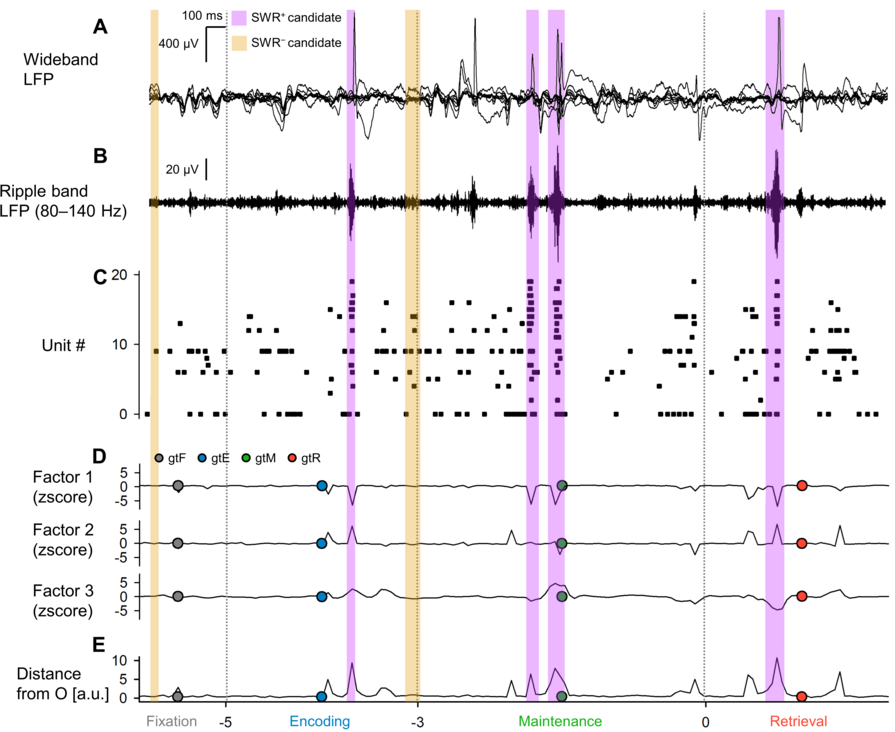
\includegraphics[width=1\textwidth]{./src/figures/.png/Figure_ID_01.png}
        	\caption{\textbf{
Local field potential (LFP), multiunit activity, and neural trajectory of the hippocampus during a modified Sternberg task
}
\smallskip
\\
\textbf{\textit{A.}} Representative wideband LFP traces iEEG signals recorded in the left hippocampal head. The subject conducted a modified Sternberg working memory task, including fixation (1 s, \textit{gray}), encoding (2 s, \textit{blue}), maintenance (3 s, \textit{green}), and retrieval (2 s, \textit{red}). \textbf{\textit{B.}} The corresponding ripple band LFP traces. \textbf{\textit{C.}} The raster plot of multiunit spikes estimated from the LFP traces using a spike sorting algorithm \cite{niediek_reliable_2016}. \textbf{\textit{D.}} Neural trajectory calculated by GPFA on spike counts per unit with 50-ms bins. The dot circles show the coordinate of geometric median for each phase. \textbf{\textit{E.}} Trajectory distance from the origin $O$. Note that \textit{purple} and \textit{yellow} rectangles shows the timings for SWR$^+$ candidates and SWR$^-$ candidates (control for SWR$^+$), respectively.
}
% width=1\textwidth
        	\label{fig:01}
        \end{figure*}
        \clearpage
        \begin{figure*}[ht]
            \pdfbookmark[2]{ID 02}{figure_id_02}
        	\centering
            \includegraphics[width=0.5\textwidth]{./src/figures/.png/Figure_ID_02.png}
        	\caption{\textbf{
State-dependent hippocampal neural trajectory
}
\smallskip
\\
\textbf{\textit{A.}} Neural trajectory in the first three-dimensional factors calculated by GPFA. Smaller dots indicate coordinates of 50-ms neural trajectory bins. Larger dots with \textit{black} edges represent geometric medians for the following phases in the Sternberg working memory task: fixation (\textit{gray}), encoding (\textit{blue}), maintenance (\textit{green}), and retrieval (\textit{red}). \textbf{\textit{B.}} The log-likelihood of GPFA models in relation to the number of dimensions to embed multiunit spikes in MTL regions. Notably, the optimal dimension was identified as three using the elbow method.  \textbf{\textit{C.}}  Distance of neural trajectory from the origin ($O$) for the hippocampus (Hipp.), entorhinal cortex (EC), and amygdala (Amy.), plotted against the time from probe onset. \textbf{\textit{D.}} Trajectory distance from $O$ in MTL regions, with the hippocampus showing the greatest distance, followed by the EC and the Amygdala. \textbf{\textit{E.}}  Inter-phase trajectory distances in the MTL regions.
Abbreviations:
}
% width=0.5\textwidth
        	\label{fig:02}
        \end{figure*}
        \clearpage
        \begin{figure*}[ht]
            \pdfbookmark[2]{ID 03}{figure_id_03}
        	\centering
            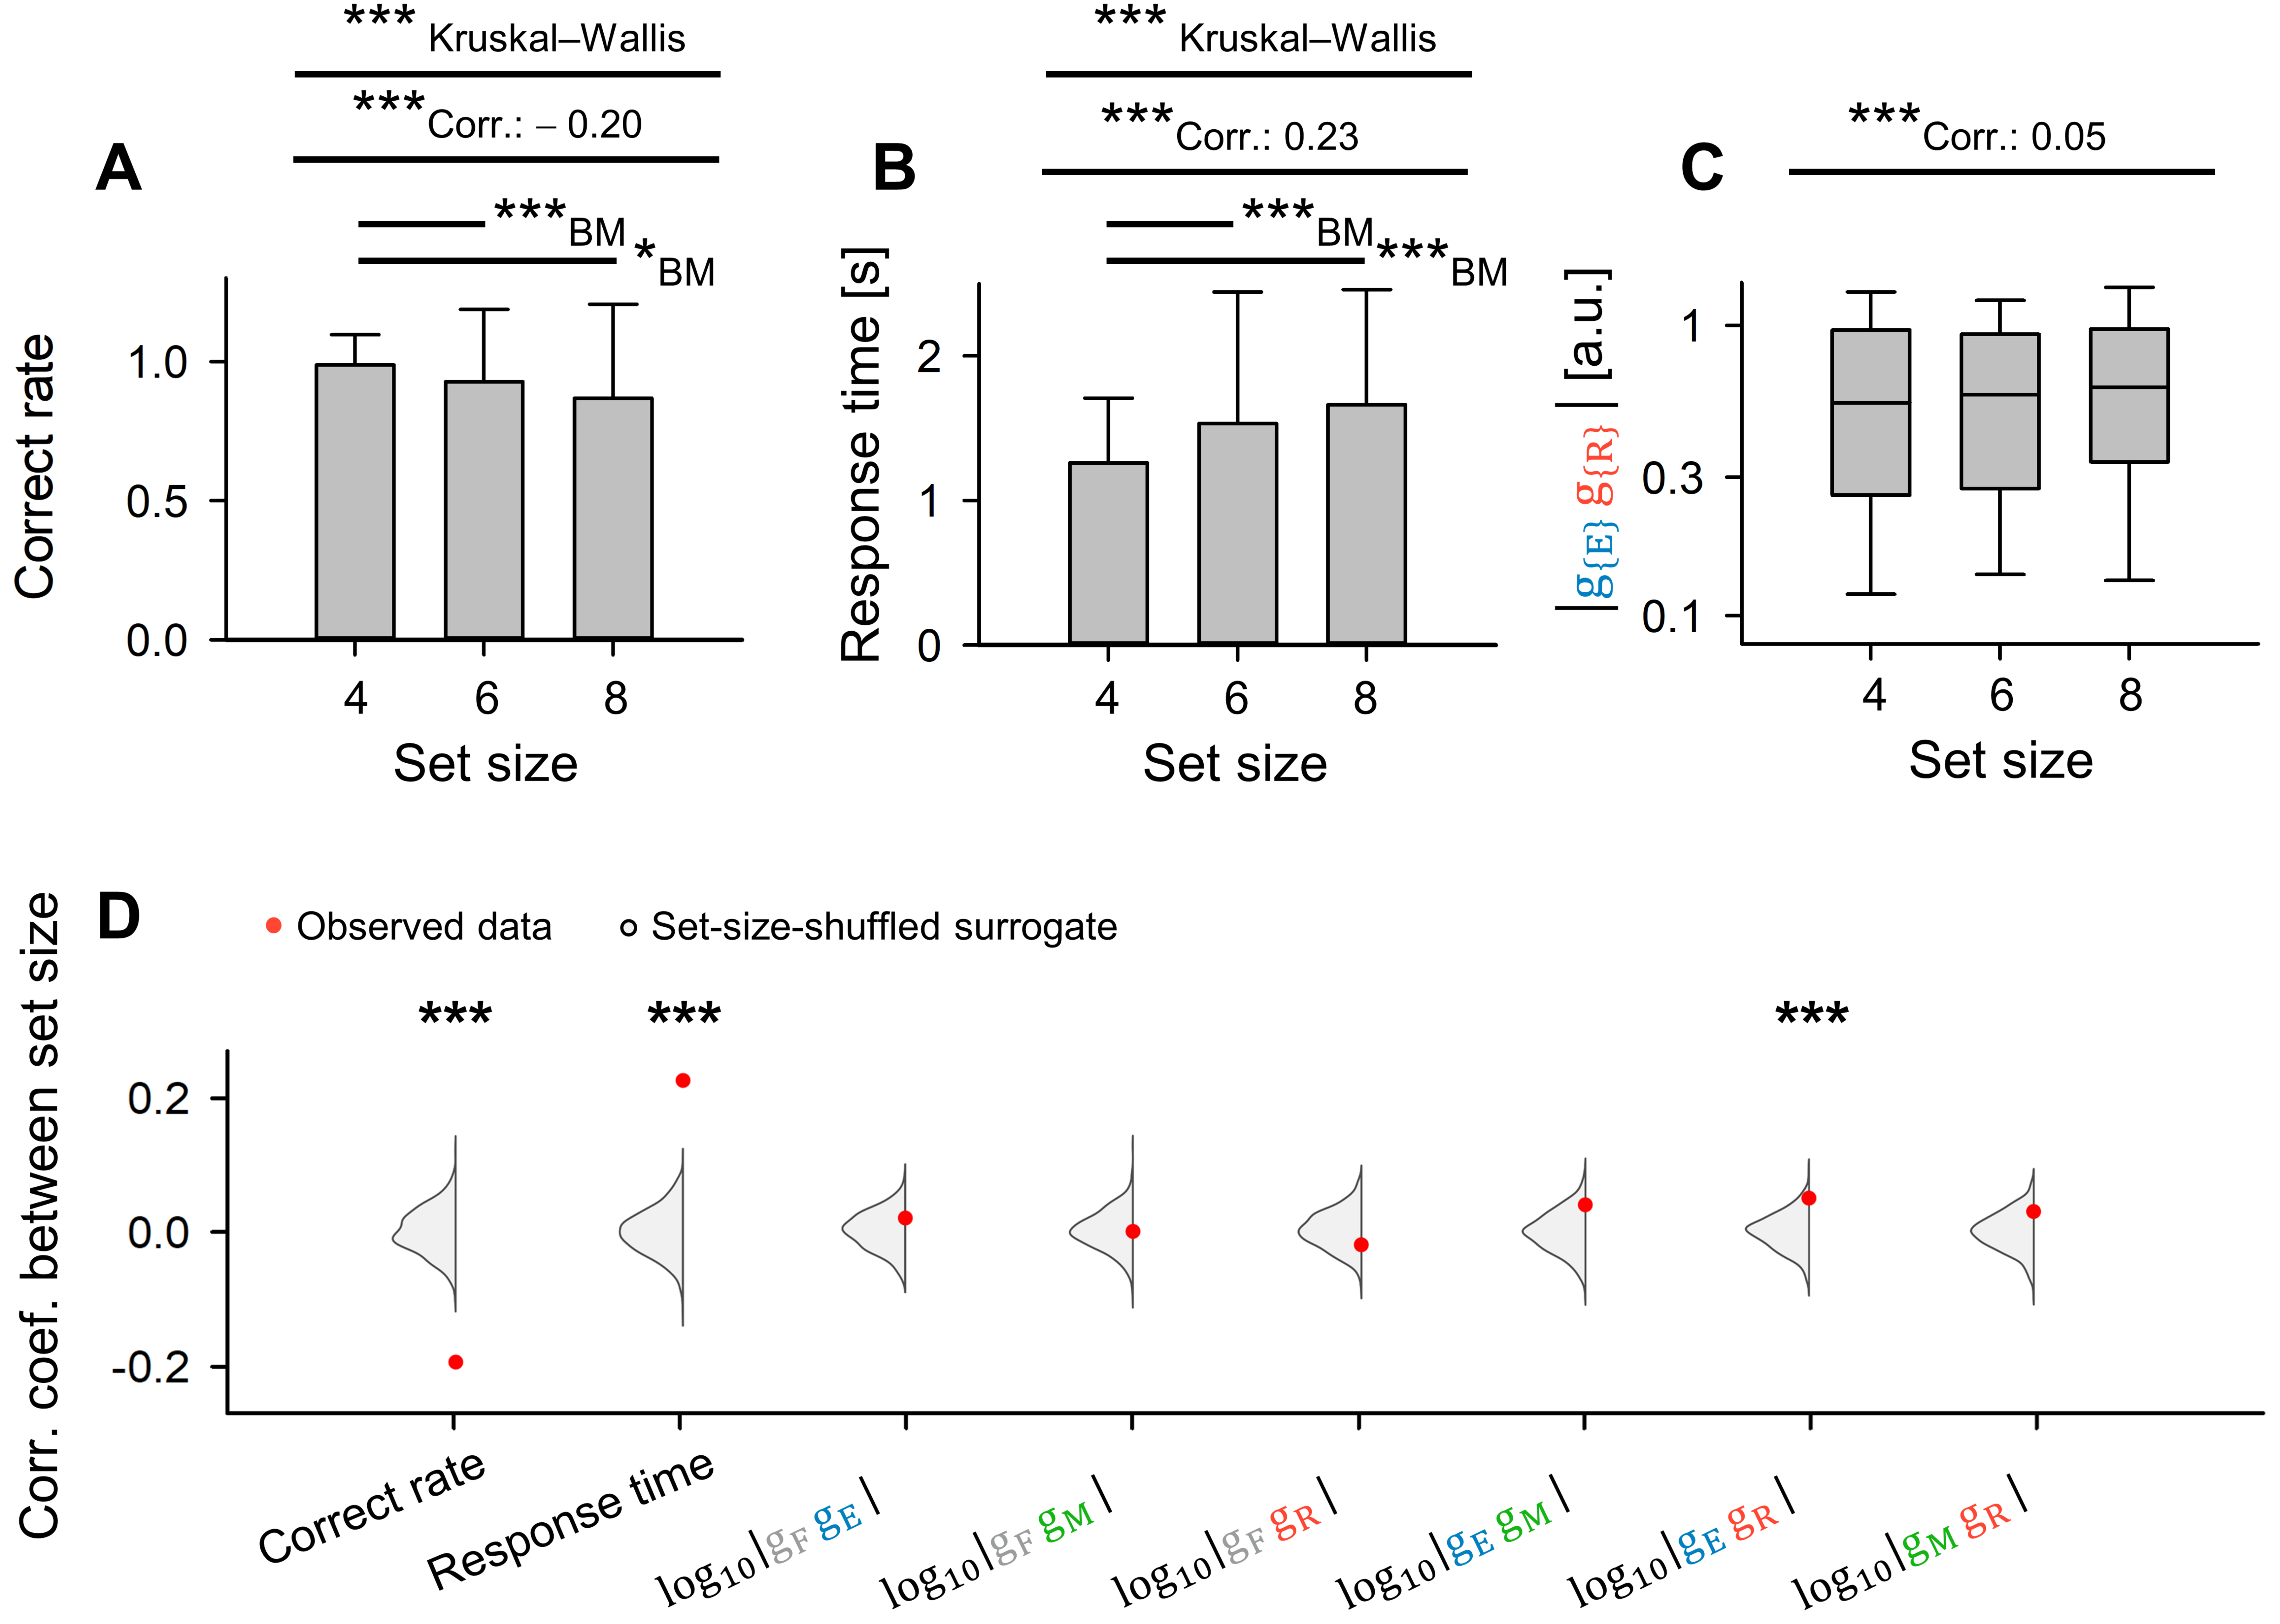
\includegraphics[width=1\textwidth]{./src/figures/.png/Figure_ID_03.png}
        	\caption{\textbf{
Memory-load dependency in trajectory distance between encoding and retrieval states in the hippocampus 
}
\smallskip
\\
\textbf{\textit{A.}} Set size (number of letters to encode) and correct rate in the WM task (coefficient = $-0.20$, ***\textit{p} $<$ 0.001). \textbf{\textit{B.}} Set size and response time (coefficient = 0.23, ***\textit{p} $<$ 0.001).  \textbf{\textit{C.}} Set size and the inter-phase distances between encoding and retrieval phases ($\lVert \mathrm{g_{E}g_{R}} \rVert$) (correlation coefficient = 0.05). \textbf{\textit{D.}} \textit{Red} dots show experimentally observed correlations between set size and the following parameters: correct rate, response time, $\log_{10}{\lVert \mathrm{g_{F}g_{E}} \rVert}$, $\log_{10}{\lVert \mathrm{g_{F}g_{M}} \rVert}$, $\log_{10}{\lVert \mathrm{g_{F}g_{R}} \rVert}$, $\log_{10}{\lVert \mathrm{g_{E}g_{M}} \rVert}$, $\log_{10}{\lVert \mathrm{g_{E}g_{R}} \rVert}$, and $\log_{10}{\lVert \mathrm{g_{M}g_{R}} \rVert}$. The \textit{gray} kernel density plot shows corresponding set-size-shuffled surrogate (\textit{n} = 1,000) (***\textit{p}s $<$ 0.001).
}
% width=1\textwidth
        	\label{fig:03}
        \end{figure*}
        \clearpage
        \begin{figure*}[ht]
            \pdfbookmark[2]{ID 04}{figure_id_04}
        	\centering
            \includegraphics[width=1\textwidth]{./src/figures/.png/Figure_ID_04.png}
        	\caption{\textbf{
SWR detection in putative CA1 regions
}
\smallskip
\\
\textbf{\textit{A.}} Two-dimensional UMAP (uniform manifold approximation and projection)\cite{mcinnes_umap_2018} projection of multiunit spikes during SWR$^+$ candidates (\textit{purple}) and SWR$^-$ candidates (\textit{yellow}). \textbf{\textit{B.}}  Cumulative density plot of silhouette scores, a barometer for UMAP clustering quality, for hippocampal regions (refer to Table 2). Note that hippocampal regions with silhouette scores exceeding 0.60 (= $75^{th}$ percentile) were defined as putative CA1 regions. SWR$^+$ and SWR$^-$ candidates recorded in these putative CA1 regions were defined as SWR$^+$ and SWR$^-$ (\textit{n}s = 1,170), respectively. \textbf{\textit{C.}}  The distributions of durations for SWR$^+$ (\textit{purple}) and SWR$^-$ (\textit{yellow}), which are identical due to their definitions (93.0 [65.4] ms, median [IQR]). \textbf{\textit{D.}}  SWR incidence for both SWR$^+$ (\textit{purple}) and SWR$^-$ (\textit{yellow}) relative to time from probe, represented as mean \textpm 95\% confidence interval, although the intervals might not be visible due to their narrow range. Note the significant elevation in SWR incidence was detected during the first 400 ms of the retrieval phase (0.421 [Hz], *\textit{p} $<$ 0.05, bootstrap test). \textbf{\textit{E.}}  The distributions of ripple band peak amplitude for SWR$^-$ (\textit{yellow}; 2.37 [0.33] SD of baseline, median [IQR]) and SWR$^+$ (\textit{purple}; 3.05 [0.85] SD of baseline, median [IQR]) (***\textit{p} $<$ 0.001, the Brunner--Munzel test).
}
% width=1\textwidth
        	\label{fig:04}
        \end{figure*}
        \clearpage
        \begin{figure*}[ht]
            \pdfbookmark[2]{ID 05}{figure_id_05}
        	\centering
            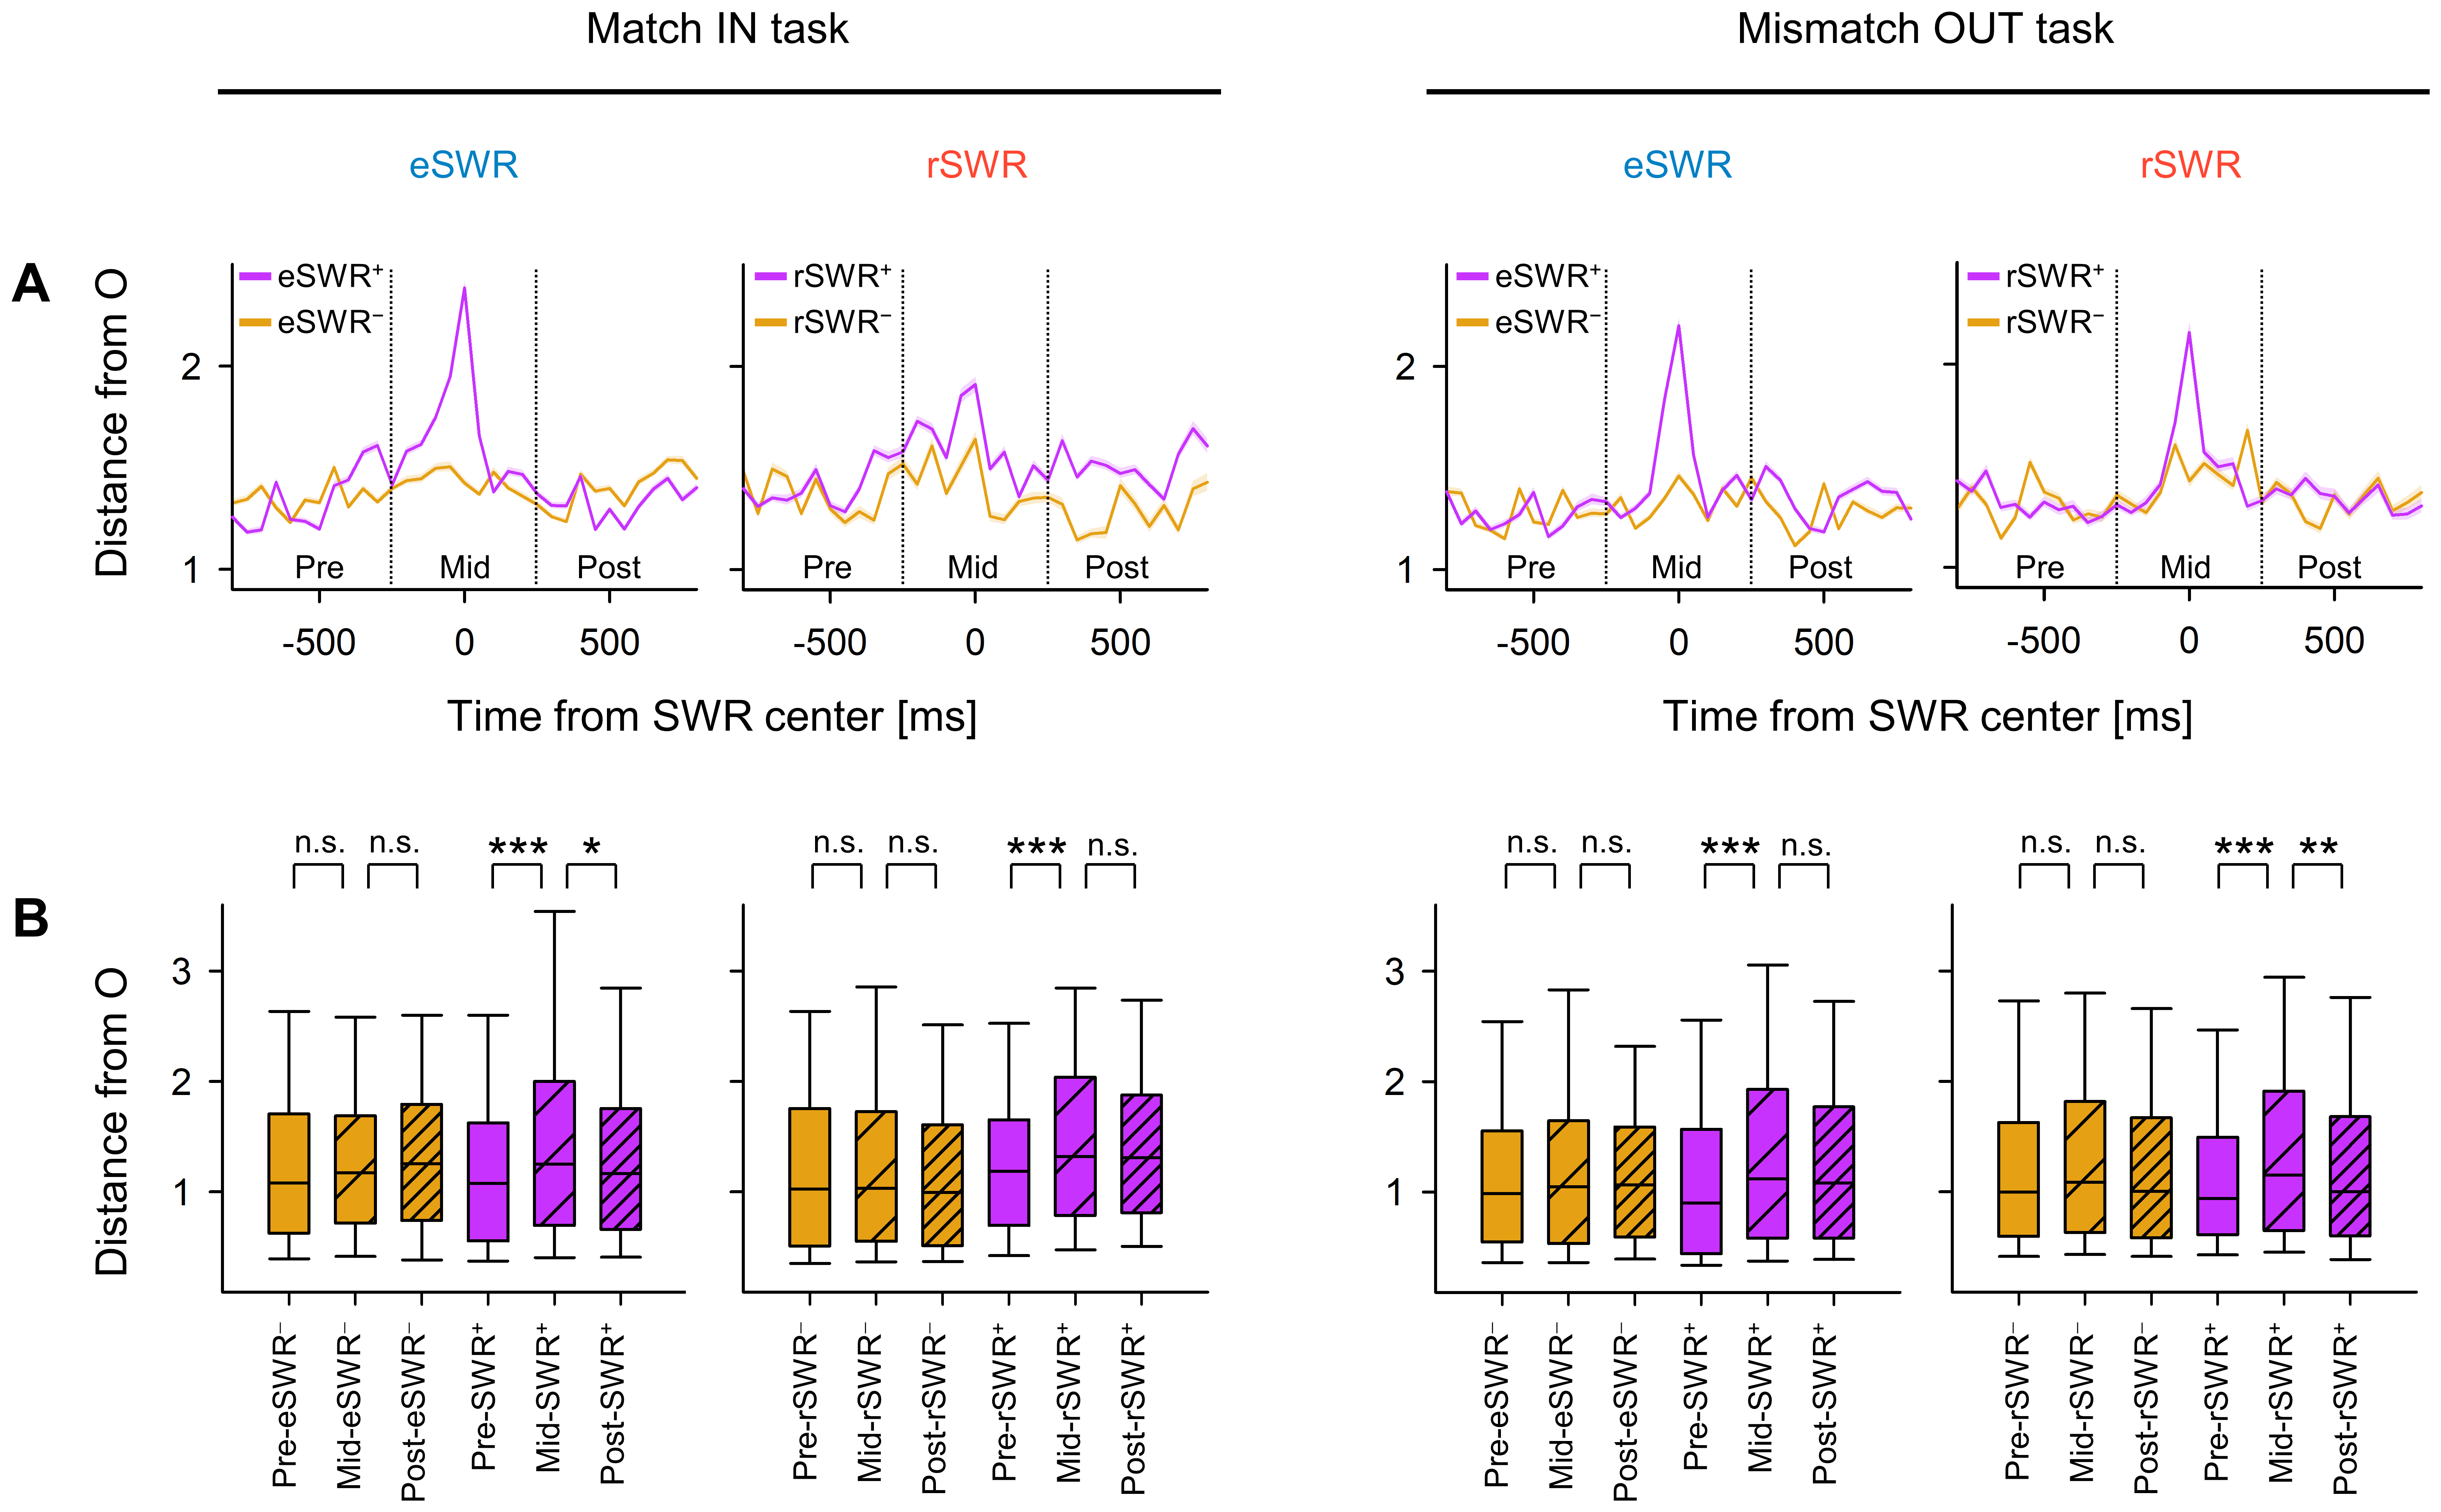
\includegraphics[width=1\textwidth]{./src/figures/.png/Figure_ID_05.png}
        	\caption{\textbf{
Transient neural trajectory change during SWR
}
\smallskip
\\
\textbf{\textit{A.}} Distance from the origin ($O$) of the peri-sharp-wave-ripple trajectory (mean \textpm 95\% confidence interval, although the intervals might not be visible due to their narrow ranges. \textbf{\textit{B.}}  The distance from the origin ($O$) during pre-, mid-, and post-SWR periods (*\textit{p} $<$ 0.05, **\textit{p} $<$ 0.01, ***\textit{p} $<$ 0.001; Brunner--Munzel test). Abbreviations: SWR, sharp-wave ripple events; eSWR, SWR during the encoding phase; rSWR, SWR during the retrieval phase, SWR$^+$, SWR event; SWR$^-$ control events for SWR$^+$; pre-, mid-, or post-SWR, the time interval from $-800$ to $-250$ ms, from $-250$ to $+250$ ms, or from $+250$ to $+800$ ms relative to SWR center.
}
% width=1\textwidth
        	\label{fig:05}
        \end{figure*}
        \clearpage
        \begin{figure*}[ht]
            \pdfbookmark[2]{ID 06}{figure_id_06}
        	\centering
            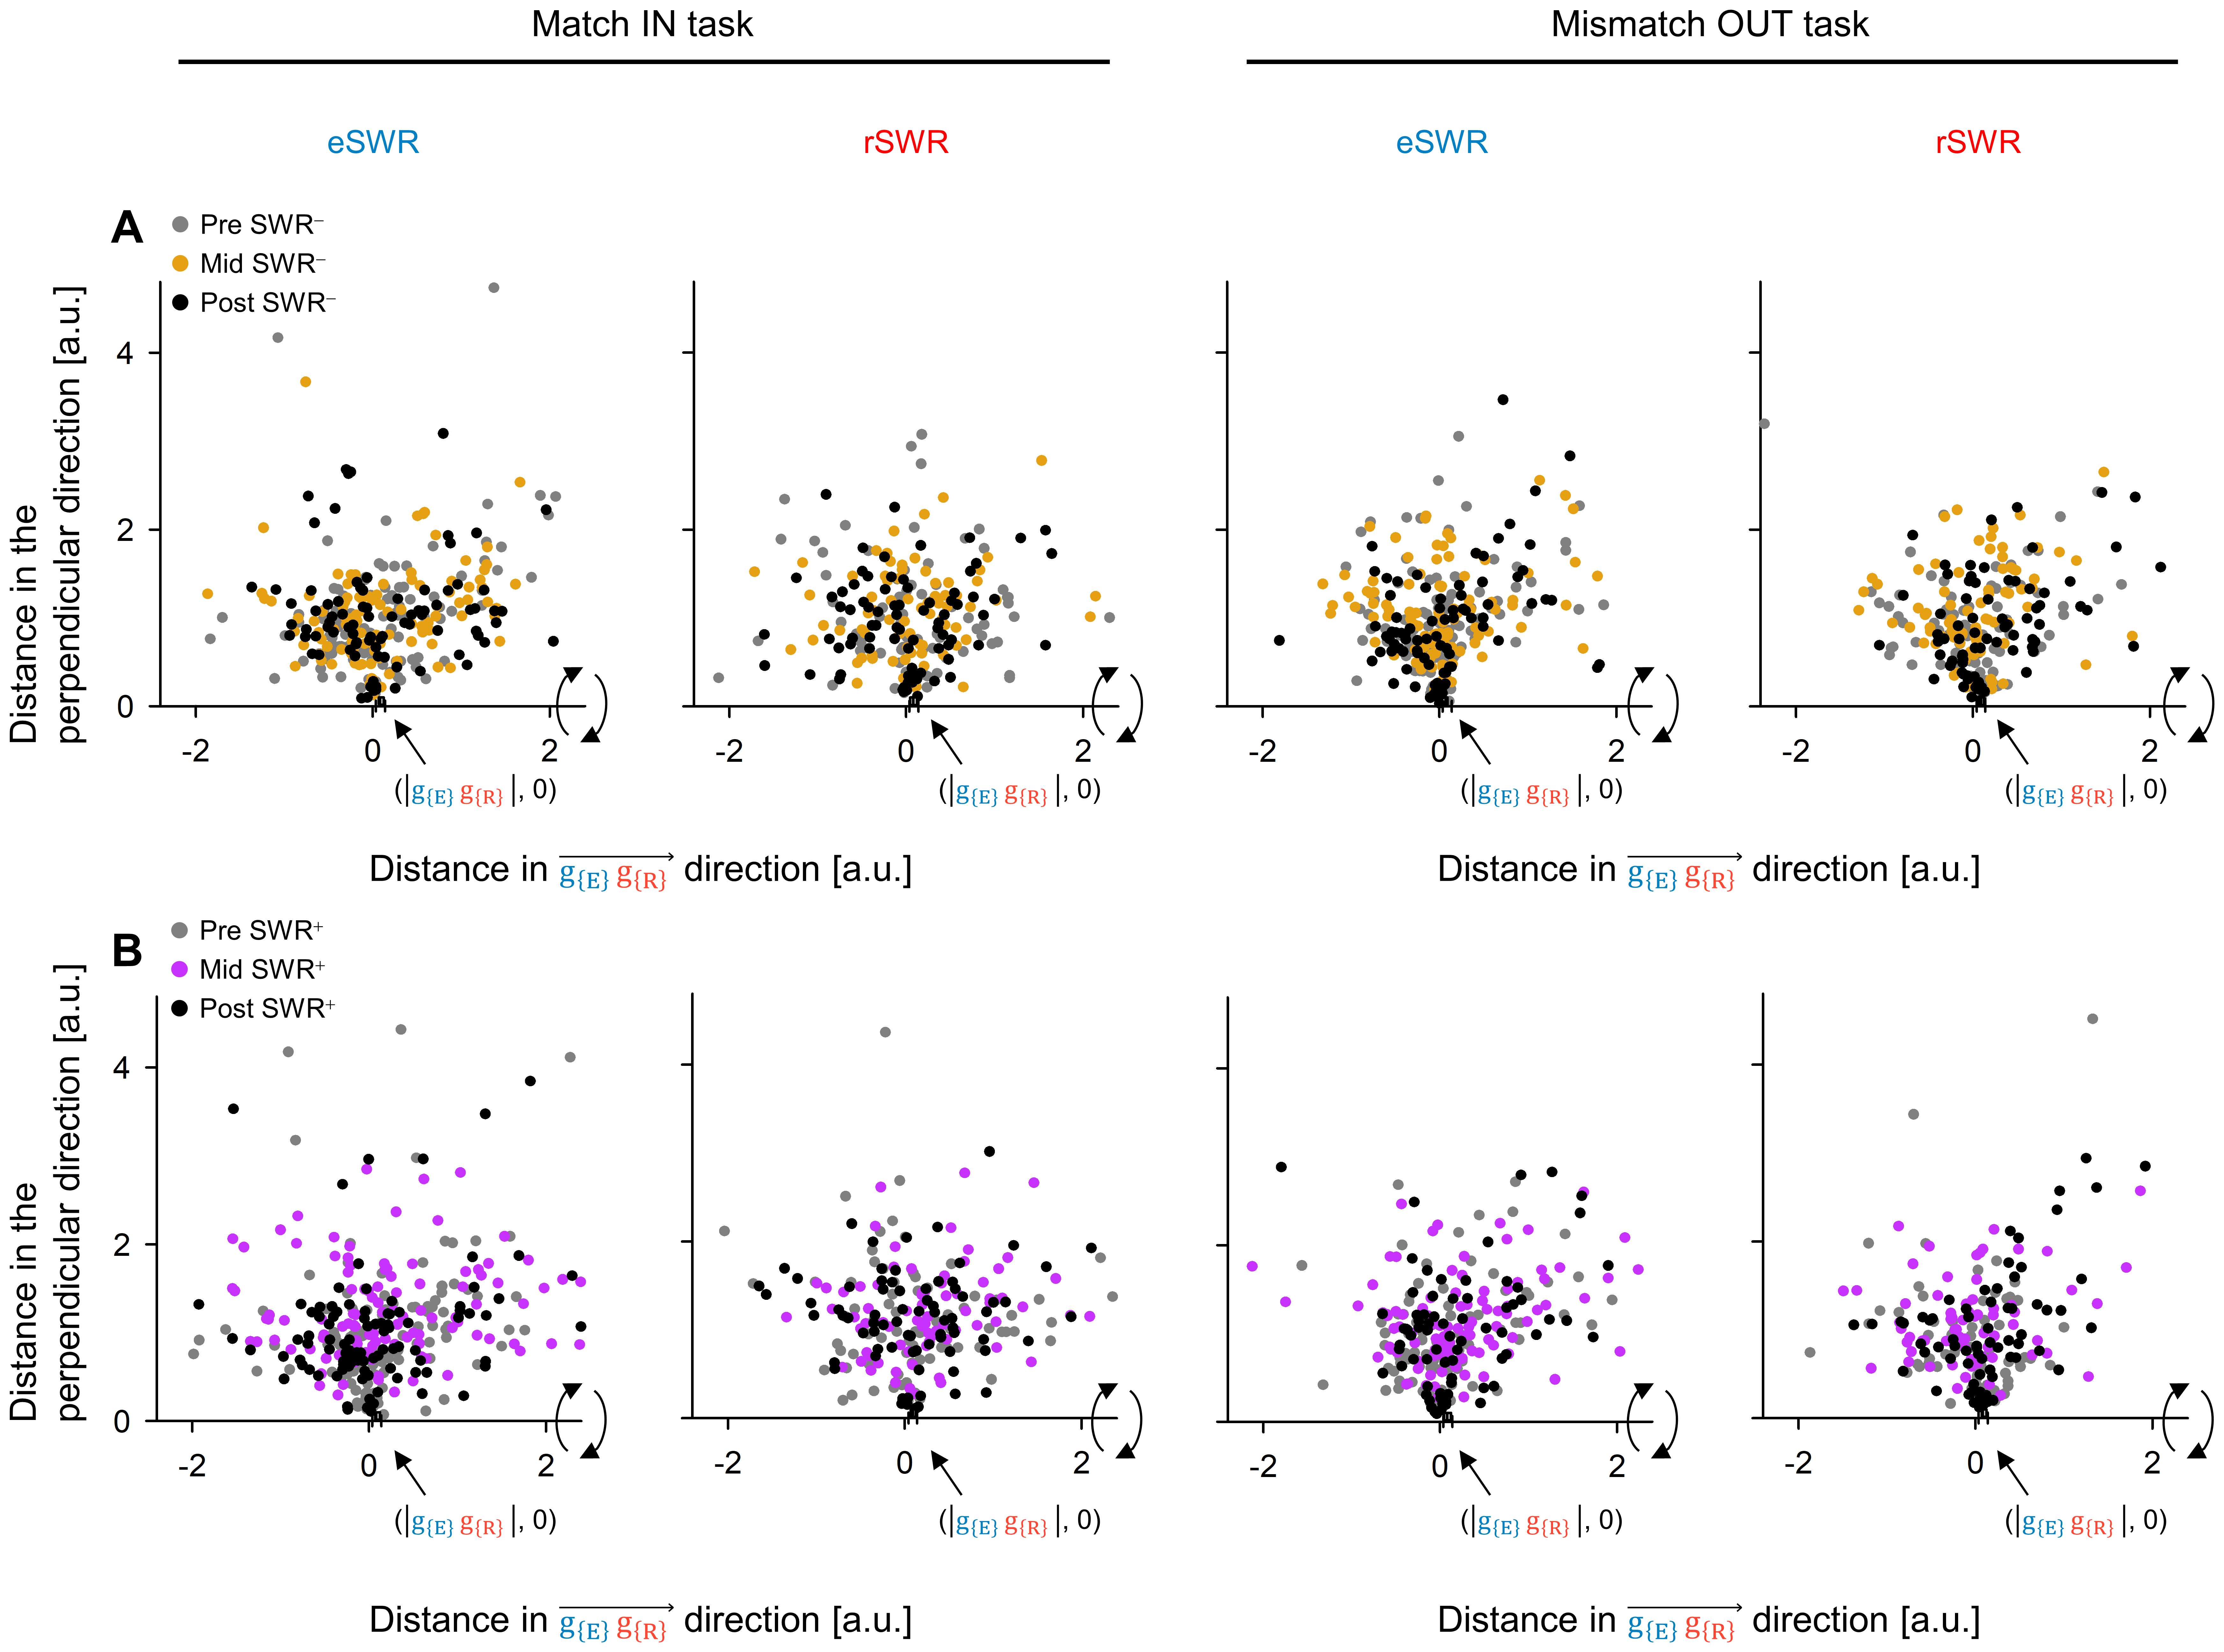
\includegraphics[width=1\textwidth]{./src/figures/.png/Figure_ID_06.png}
        	\caption{\textbf{
Visualization of neural trajectory during SWR in two-dimensional spaces
}
\smallskip
\\
Panels show hippocampal neural trajectories during SWR, which were projected into two-dimensional spaces. \textbf{\textit{A.}} Hippocampal neural trajectories during pre- (\textit{gray}), mid- (\textit{yellow}), and post-SWR$^-$ (\textit{black}). \textbf{\textit{B.}} The equivalents for SWR$^+$, instead of SWR$^-$. The $\lVert \mathrm{g_{E}g_{R}} \rVert$ varied across sessions. The projection was applied as follows. First, linear transformation was applied in the way that $\mathrm{g_{E}}$ was placed at the origin $O$ (0, 0), and $\mathrm{g_{R}}$ at ($\lVert \mathrm{g_{E}g_{R}} \rVert$, 0). Moreover, point cloud was rotated around the $\mathrm{g_{E}g_{R}}$ axis (= x axis) to fit in two-dimensional spaces. Thus, in these two-dimensional spaces, both the distances from $O$ and angles between the $\mathrm{g_{E}g_{R}}$ axis are preserved from the original three dimensional spaces. Abbreviations: SWR, sharp-wave ripple events; eSWR, SWR during the encoding phase; rSWR, SWR during the retrieval phase, SWR$^+$, SWR event; SWR$^-$ control events for SWR$^+$; pre-SWR, mid-SWR, or post-SWR, the time interval from $-800$ to $-250$ ms, from $-250$ to $+250$ ms, or from $+250$ to $+800$ ms from the center of SWR. 
}
% width=1\textwidth
        	\label{fig:06}
        \end{figure*}
        \clearpage
        \begin{figure*}[ht]
            \pdfbookmark[2]{ID 07}{figure_id_07}
        	\centering
            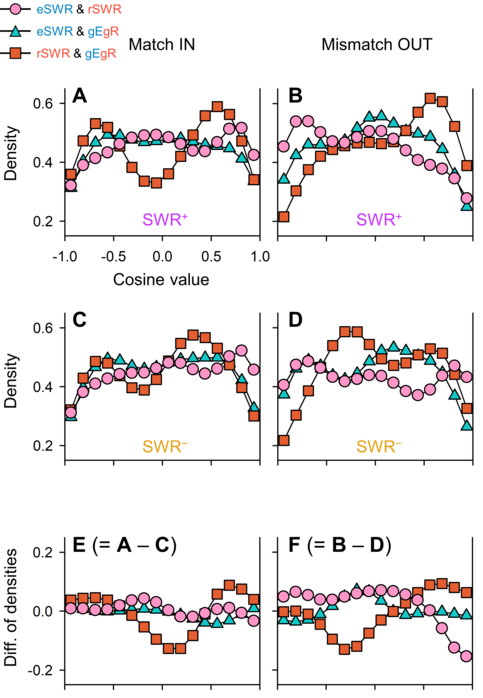
\includegraphics[width=0.5\textwidth]{./src/figures/.png/Figure_ID_07.png}
        	\caption{\textbf{
Neural trajectory directions of SWR based on encoding and retrieval states
}
\smallskip
\\
\textbf{\textit{A--B}} Kernel density estimation (KDE) distribution of $\protect\overrightarrow{{\mathrm{eSWR^+}}} \cdot \protect\overrightarrow{{\mathrm{rSWR^+}}}$ (\textit{pink circles}), $\protect\overrightarrow{{\mathrm{eSWR^+}}} \cdot \protect\overrightarrow{{\mathrm{g_{E}g_{R}}}}$ (\textit{blue triangles}), and $\protect\overrightarrow{{\mathrm{rSWR^+}}} \cdot \protect\overrightarrow{{\mathrm{g_{E}g_{R}}}}$ (\textit{red rectangles}) in Match In (\textit{A}) and Mismatch OUT task (\textit{B}). \textbf{\textit{C--D.}} The corresponding distributions of $\mathrm{SWR^-}$ instead of those of $\mathrm{SWR^+}$ in \textit{A--B}. \textbf{\textit{E--F.}} The differences in distributions of $\mathrm{SWR^+}$ and $\mathrm{SWR^-}$, highlighting the SWR components (\textit{E} = \textit{C} $-$ \textit{A}; \textit{F} = \textit{B} $-$ \textit{D}). Note the biphasic distributions of $\protect\overrightarrow{{\mathrm{rSWR^-}}} \cdot \protect\overrightarrow{{\mathrm{g_{E}g_{R}}}}$, indicating neural fluctuation betwen the encoding and retrieval states during the Sternberg task. Additionally, in Mismatch OUT task, inverse directionality between $\protect\overrightarrow{{\mathrm{eSWR^+}}}$ and $\protect\overrightarrow{{\mathrm{rSWR^+}}}$ (\textit{pink circles}) was found, though not in Match IN task \textbf{\textit{E--F}}). Last, shifts from the retrieval to encoding states were observed for SWR components both in Match IN and Mismatch OUT tasks (\textit{red rectangles} in \textit{E--F}).
}
% width=0.5\textwidth
        	\label{fig:07}
        \end{figure*}
        \clearpage
        \begin{figure*}[ht]
            \pdfbookmark[2]{ID 01}{figure_id_01}
        	\centering
            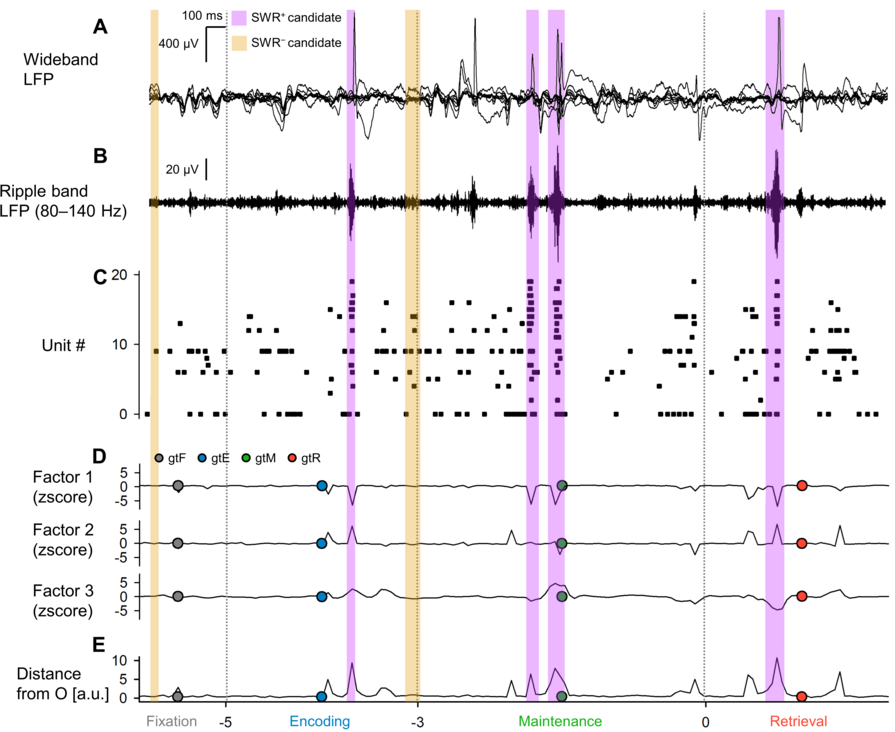
\includegraphics[width=1\textwidth]{./src/figures/.png/Figure_ID_01.png}
        	\caption{\textbf{
Local field potential (LFP), multiunit activity, and neural trajectory of the hippocampus during a modified Sternberg task
}
\smallskip
\\
\textbf{\textit{A.}} Representative wideband LFP traces iEEG signals recorded in the left hippocampal head. The subject conducted a modified Sternberg working memory task, including fixation (1 s, \textit{gray}), encoding (2 s, \textit{blue}), maintenance (3 s, \textit{green}), and retrieval (2 s, \textit{red}). \textbf{\textit{B.}} The corresponding ripple band LFP traces. \textbf{\textit{C.}} The raster plot of multiunit spikes estimated from the LFP traces using a spike sorting algorithm \cite{niediek_reliable_2016}. \textbf{\textit{D.}} Neural trajectory calculated by GPFA on spike counts per unit with 50-ms bins. The dot circles show the coordinate of geometric median for each phase. \textbf{\textit{E.}} Trajectory distance from the origin $O$. Note that \textit{purple} and \textit{yellow} rectangles shows the timings for SWR$^+$ candidates and SWR$^-$ candidates (control for SWR$^+$), respectively.
}
% width=1\textwidth
        	\label{fig:01}
        \end{figure*}
        \clearpage
        \begin{figure*}[ht]
            \pdfbookmark[2]{ID 02}{figure_id_02}
        	\centering
            \includegraphics[width=0.5\textwidth]{./src/figures/.png/Figure_ID_02.png}
        	\caption{\textbf{
State-dependent hippocampal neural trajectory
}
\smallskip
\\
\textbf{\textit{A.}} Neural trajectory in the first three-dimensional factors calculated by GPFA. Smaller dots indicate coordinates of 50-ms neural trajectory bins. Larger dots with \textit{black} edges represent geometric medians for the following phases in the Sternberg working memory task: fixation (\textit{gray}), encoding (\textit{blue}), maintenance (\textit{green}), and retrieval (\textit{red}). \textbf{\textit{B.}} The log-likelihood of GPFA models in relation to the number of dimensions to embed multiunit spikes in MTL regions. Notably, the optimal dimension was identified as three using the elbow method.  \textbf{\textit{C.}}  Distance of neural trajectory from the origin ($O$) for the hippocampus (Hipp.), entorhinal cortex (EC), and amygdala (Amy.), plotted against the time from probe onset. \textbf{\textit{D.}} Trajectory distance from $O$ in MTL regions, with the hippocampus showing the greatest distance, followed by the EC and the Amygdala. \textbf{\textit{E.}}  Inter-phase trajectory distances in the MTL regions.
Abbreviations:
}
% width=0.5\textwidth
        	\label{fig:02}
        \end{figure*}
        \clearpage
        \begin{figure*}[ht]
            \pdfbookmark[2]{ID 03}{figure_id_03}
        	\centering
            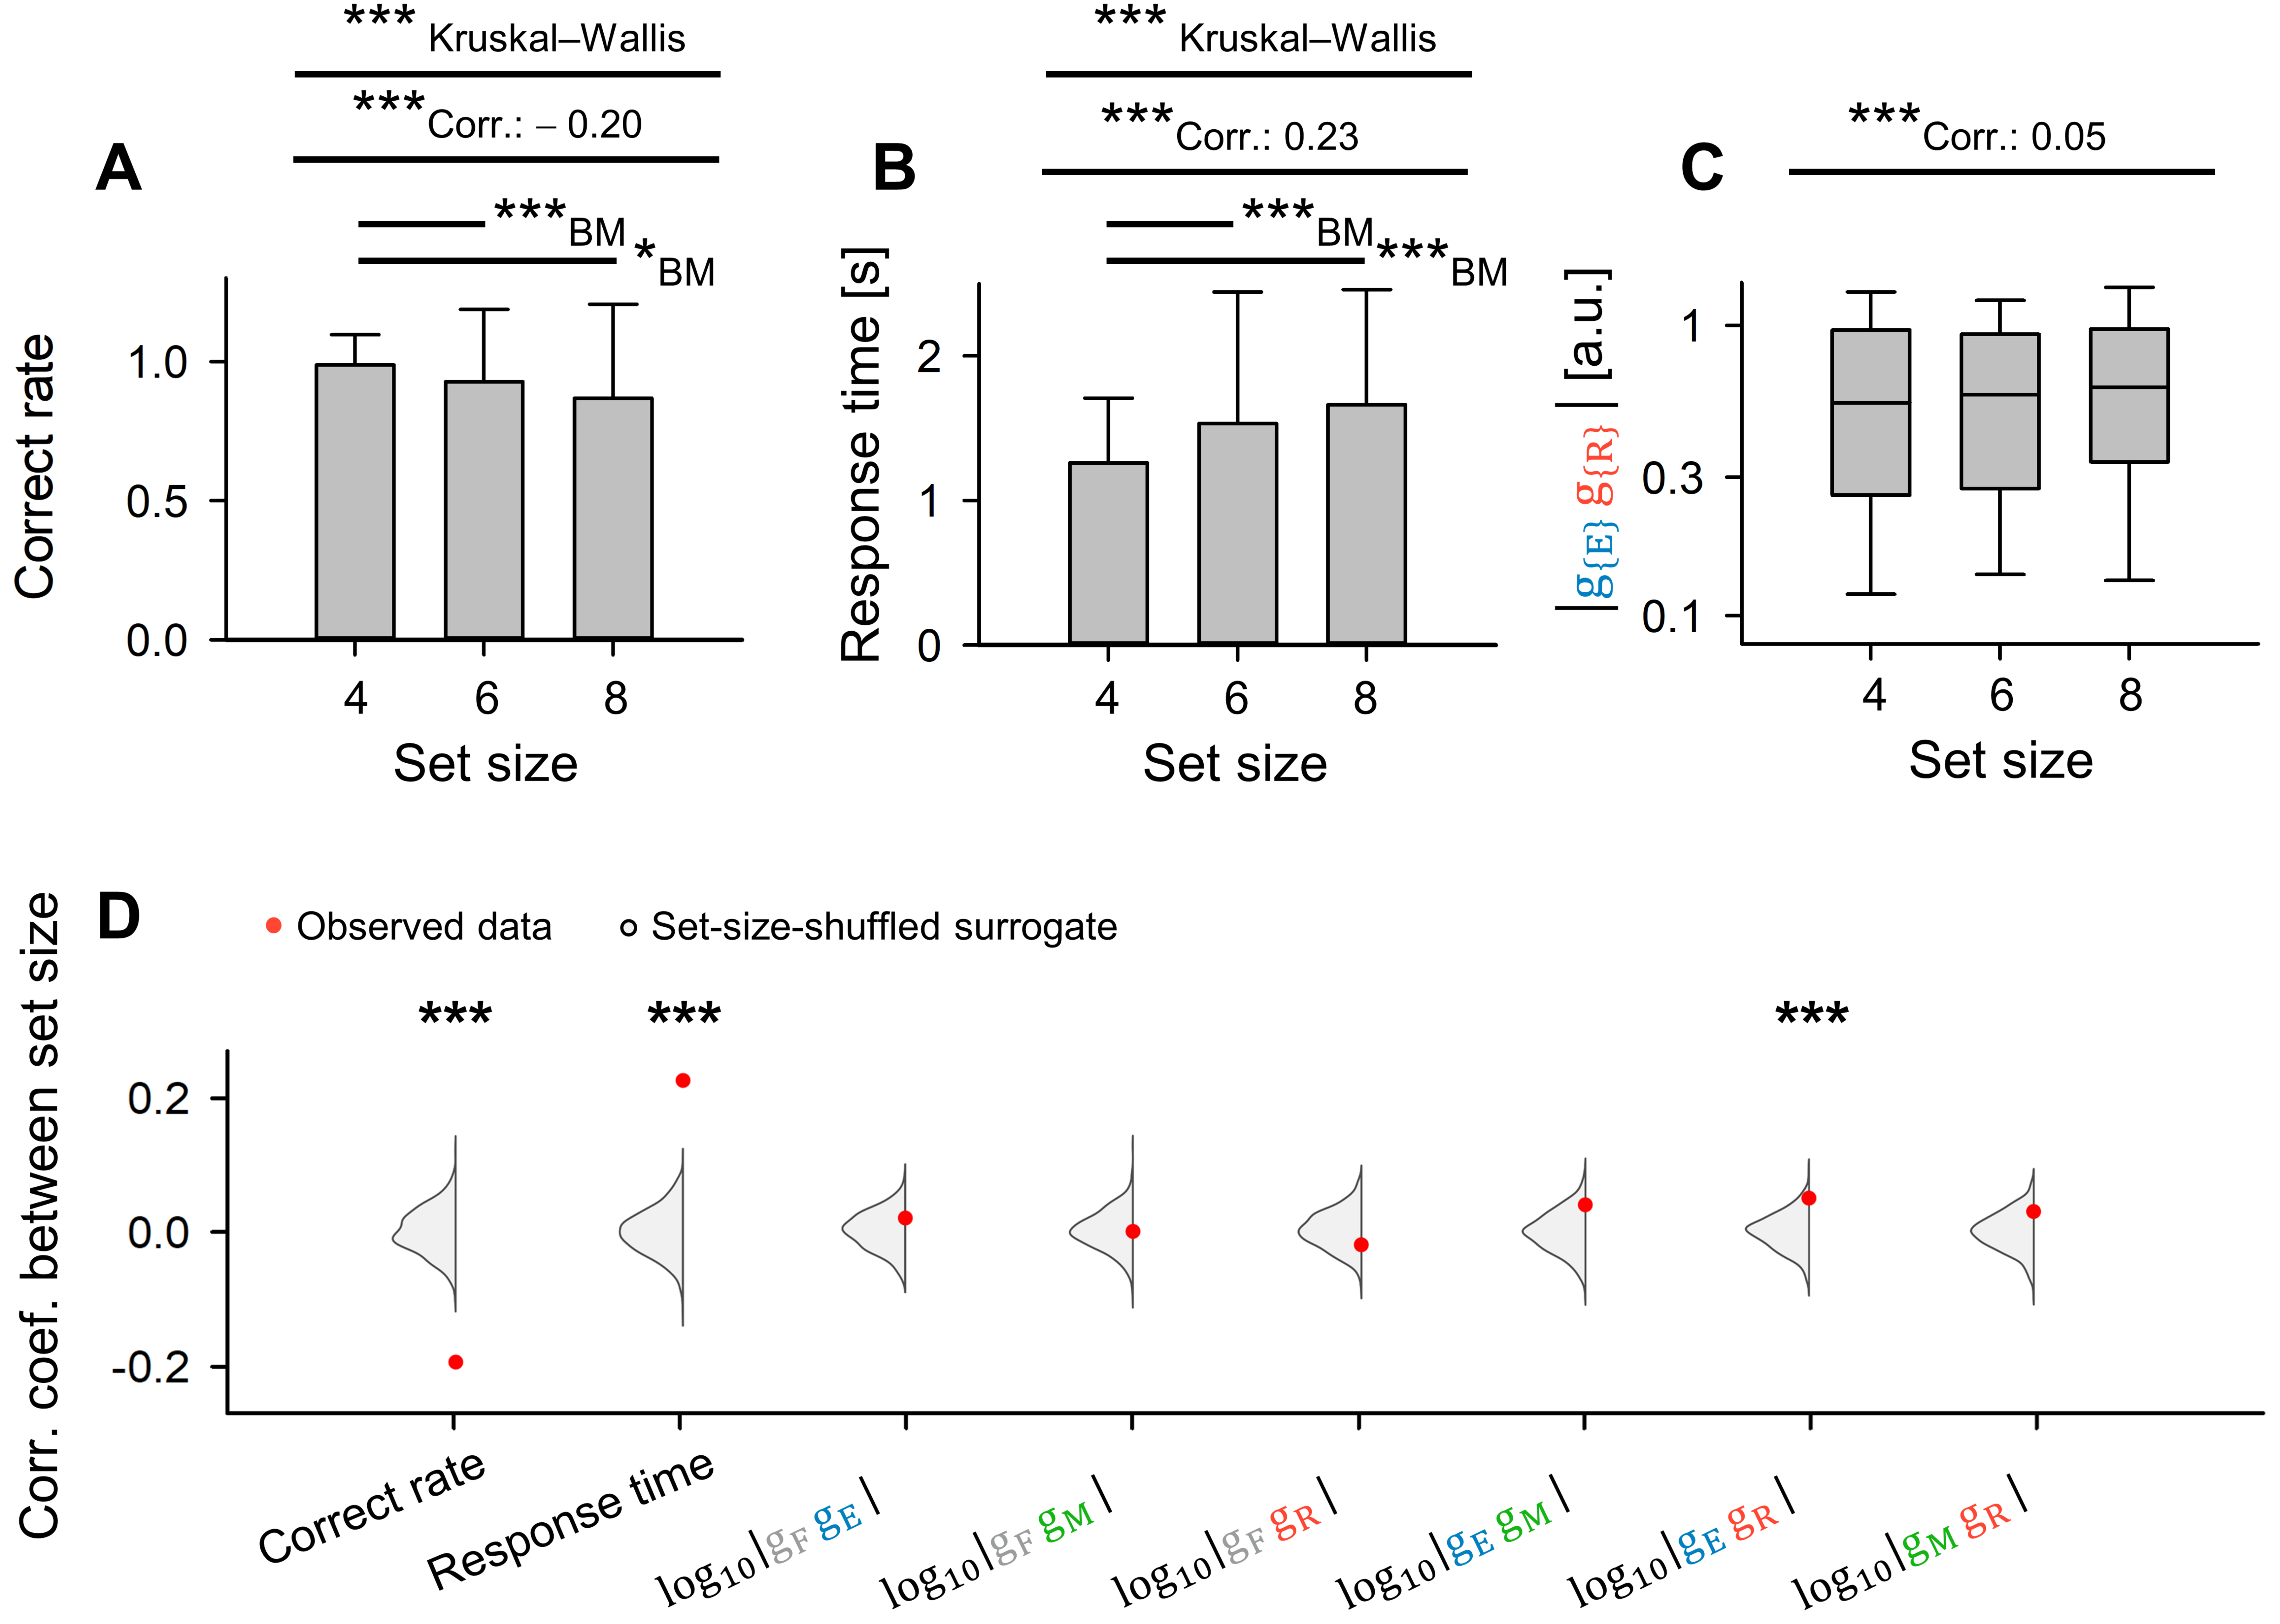
\includegraphics[width=1\textwidth]{./src/figures/.png/Figure_ID_03.png}
        	\caption{\textbf{
Memory-load dependency in trajectory distance between encoding and retrieval states in the hippocampus 
}
\smallskip
\\
\textbf{\textit{A.}} Set size (number of letters to encode) and correct rate in the WM task (coefficient = $-0.20$, ***\textit{p} $<$ 0.001). \textbf{\textit{B.}} Set size and response time (coefficient = 0.23, ***\textit{p} $<$ 0.001).  \textbf{\textit{C.}} Set size and the inter-phase distances between encoding and retrieval phases ($\lVert \mathrm{g_{E}g_{R}} \rVert$) (correlation coefficient = 0.05). \textbf{\textit{D.}} \textit{Red} dots show experimentally observed correlations between set size and the following parameters: correct rate, response time, $\log_{10}{\lVert \mathrm{g_{F}g_{E}} \rVert}$, $\log_{10}{\lVert \mathrm{g_{F}g_{M}} \rVert}$, $\log_{10}{\lVert \mathrm{g_{F}g_{R}} \rVert}$, $\log_{10}{\lVert \mathrm{g_{E}g_{M}} \rVert}$, $\log_{10}{\lVert \mathrm{g_{E}g_{R}} \rVert}$, and $\log_{10}{\lVert \mathrm{g_{M}g_{R}} \rVert}$. The \textit{gray} kernel density plot shows corresponding set-size-shuffled surrogate (\textit{n} = 1,000) (***\textit{p}s $<$ 0.001).
}
% width=1\textwidth
        	\label{fig:03}
        \end{figure*}
        \clearpage
        \begin{figure*}[ht]
            \pdfbookmark[2]{ID 01}{figure_id_01}
        	\centering
            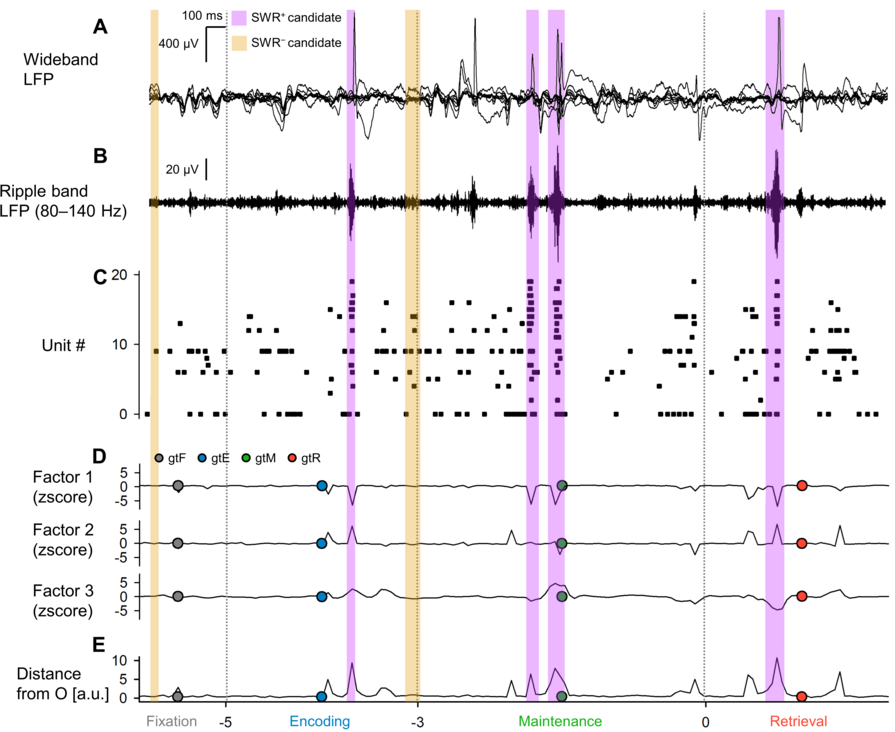
\includegraphics[width=1\textwidth]{./src/figures/.png/Figure_ID_01.png}
        	\caption{\textbf{
Local field potential (LFP), multiunit activity, and neural trajectory of the hippocampus during a modified Sternberg task
}
\smallskip
\\
\textbf{\textit{A.}} Representative wideband LFP traces iEEG signals recorded in the left hippocampal head. The subject conducted a modified Sternberg working memory task, including fixation (1 s, \textit{gray}), encoding (2 s, \textit{blue}), maintenance (3 s, \textit{green}), and retrieval (2 s, \textit{red}). \textbf{\textit{B.}} The corresponding ripple band LFP traces. \textbf{\textit{C.}} The raster plot of multiunit spikes estimated from the LFP traces using a spike sorting algorithm \cite{niediek_reliable_2016}. \textbf{\textit{D.}} Neural trajectory calculated by GPFA on spike counts per unit with 50-ms bins. The dot circles show the coordinate of geometric median for each phase. \textbf{\textit{E.}} Trajectory distance from the origin $O$. Note that \textit{purple} and \textit{yellow} rectangles shows the timings for SWR$^+$ candidates and SWR$^-$ candidates (control for SWR$^+$), respectively.
}
% width=1\textwidth
        	\label{fig:01}
        \end{figure*}
        \clearpage
        \begin{figure*}[ht]
            \pdfbookmark[2]{ID 01}{figure_id_01}
        	\centering
            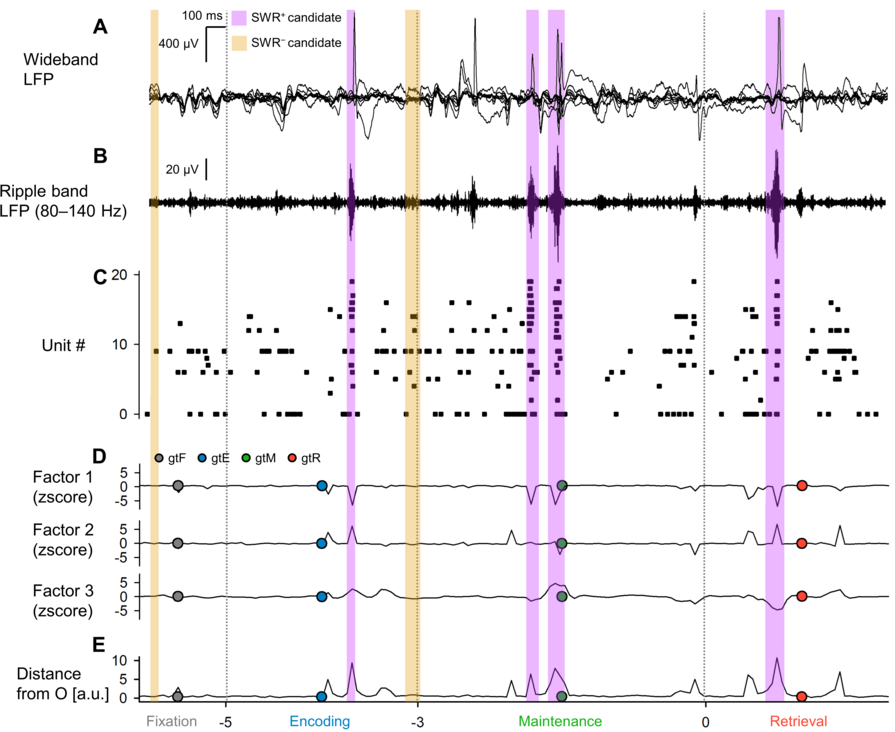
\includegraphics[width=1\textwidth]{./src/figures/.png/Figure_ID_01.png}
        	\caption{\textbf{
Local field potential (LFP), multiunit activity, and neural trajectory of the hippocampus during a modified Sternberg task
}
\smallskip
\\
\textbf{\textit{A.}} Representative wideband LFP traces iEEG signals recorded in the left hippocampal head. The subject conducted a modified Sternberg working memory task, including fixation (1 s, \textit{gray}), encoding (2 s, \textit{blue}), maintenance (3 s, \textit{green}), and retrieval (2 s, \textit{red}). \textbf{\textit{B.}} The corresponding ripple band LFP traces. \textbf{\textit{C.}} The raster plot of multiunit spikes estimated from the LFP traces using a spike sorting algorithm \cite{niediek_reliable_2016}. \textbf{\textit{D.}} Neural trajectory calculated by GPFA on spike counts per unit with 50-ms bins. The dot circles show the coordinate of geometric median for each phase. \textbf{\textit{E.}} Trajectory distance from the origin $O$. Note that \textit{purple} and \textit{yellow} rectangles shows the timings for SWR$^+$ candidates and SWR$^-$ candidates (control for SWR$^+$), respectively.
}
% width=1\textwidth
        	\label{fig:01}
        \end{figure*}
        \clearpage
        \begin{figure*}[ht]
            \pdfbookmark[2]{ID 01}{figure_id_01}
        	\centering
            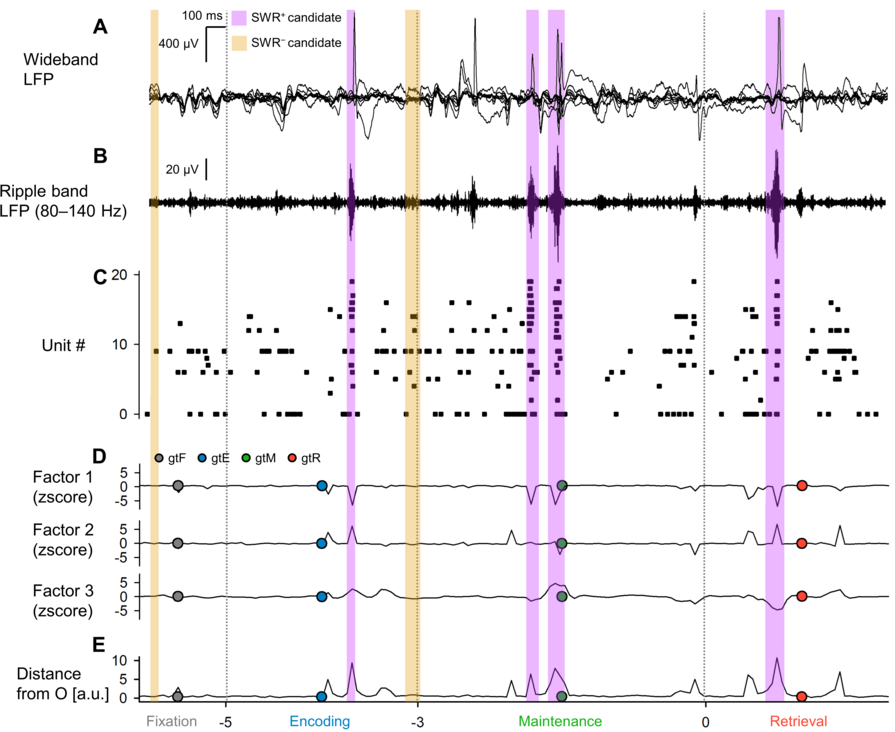
\includegraphics[width=1\textwidth]{./src/figures/.png/Figure_ID_01.png}
        	\caption{\textbf{
Local field potential (LFP), multiunit activity, and neural trajectory of the hippocampus during a modified Sternberg task
}
\smallskip
\\
\textbf{\textit{A.}} Representative wideband LFP traces iEEG signals recorded in the left hippocampal head. The subject conducted a modified Sternberg working memory task, including fixation (1 s, \textit{gray}), encoding (2 s, \textit{blue}), maintenance (3 s, \textit{green}), and retrieval (2 s, \textit{red}). \textbf{\textit{B.}} The corresponding ripple band LFP traces. \textbf{\textit{C.}} The raster plot of multiunit spikes estimated from the LFP traces using a spike sorting algorithm \cite{niediek_reliable_2016}. \textbf{\textit{D.}} Neural trajectory calculated by GPFA on spike counts per unit with 50-ms bins. The dot circles show the coordinate of geometric median for each phase. \textbf{\textit{E.}} Trajectory distance from the origin $O$. Note that \textit{purple} and \textit{yellow} rectangles shows the timings for SWR$^+$ candidates and SWR$^-$ candidates (control for SWR$^+$), respectively.
}
% width=1\textwidth
        	\label{fig:01}
        \end{figure*}


%%%%%%%%%%%%%%%%%%%%%%%%%%%%%%%%%%%%%%%%%%%%%%%%%%%%%%%%%%%%%%%%%%%%%%%%%%%%%%%%
%% Appendices
%%%%%%%%%%%%%%%%%%%%%%%%%%%%%%%%%%%%%%%%%%%%%%%%%%%%%%%%%%%%%%%%%%%%%%%%%%%%%%%%
%% \pdfbookmark[1]{Appendices}{appendices}                    
%% \appendix
%% \section{}
%% \label{}


%%%%%%%%%%%%%%%%%%%%%%%%%%%%%%%%%%%%%%%%%%%%%%%%%%%%%%%%%%%%%%%%%%%%%%%%%%%%%%%%
%% END
%%%%%%%%%%%%%%%%%%%%%%%%%%%%%%%%%%%%%%%%%%%%%%%%%%%%%%%%%%%%%%%%%%%%%%%%%%%%%%%%

\end{document}
